\documentclass[12pt,a4paper]{article}
\usepackage[utf8]{inputenc}
\usepackage[francais]{babel}
\usepackage[pdftex]{graphicx}
\usepackage{longtable}
\usepackage{amsmath}
\usepackage{amssymb}
\usepackage{float}
\usepackage{wrapfig}
\usepackage{forest}
\usepackage{listings}
\usepackage{listings-rust}
\usepackage{xcolor}
\usepackage{algorithm}
\usepackage{algpseudocode}
\edef\restoreparindent{\parindent=\the\parindent\relax}
\usepackage{parskip}
\restoreparindent
\usepackage{tikz}
\usetikzlibrary{arrows, automata}
\usepackage{subcaption}
\usepackage{graphicx}

\usepackage[export]{adjustbox}
\usepackage[T1]{fontenc}
\usepackage{hyperref}
\hypersetup{
    colorlinks,
    citecolor=blue,
    filecolor=black,
    linkcolor=black,
    urlcolor=teal,
    pdftitle={Rapport de projet de master 1 - Virgil Surin},
    pdfauthor=Virgil Surin,
    pdfpagemode=FullScreen
}
\tikzset{every picture/.style={scale=1,auto=center,every node/.style={circle, draw=black!50,fill=blue!20}}}
\graphicspath{images/}

\definecolor{codegreen}{rgb}{0,0.6,0}
\definecolor{codegray}{rgb}{0.5,0.5,0.5}
\definecolor{codepurple}{rgb}{0.58,0,0.82}
\definecolor{backcolour}{rgb}{0.95,0.95,0.92}

\lstdefinestyle{mystyle}{
    backgroundcolor=\color{backcolour},
    commentstyle=\color{codegreen},
    keywordstyle=\color{magenta},
    numberstyle=\tiny\color{blue},
    stringstyle=\color{codepurple},
    basicstyle=\ttfamily\footnotesize,
    breakatwhitespace=false,
    breaklines=true,
    captionpos=b,
    keepspaces=true,
    numbers=left,
    numbersep=5pt,
    showspaces=false,
    showstringspaces=false,
    showtabs=false,
    tabsize=2
}

\lstset{style=mystyle}

\begin{document}

% \begin{titlepage}
%   \begin{center}

%     {\Large Université de Mons}\\[1ex]
%     {\Large Faculté des sciences}\\[1ex]
%     {\Large Département d'Informatique}\\[2.5cm]

%     \newcommand{\HRule}{\rule{\linewidth}{0.3mm}}
%     % Title
%     \HRule \\[0.3cm]
%     { \LARGE \bfseries Étude comparative d'algorithmes pour énumérer les cliques d'un graphe \\[0.3cm]}
%     % { \LARGE \bfseries Rapport préliminaire de projet de Master \\[0.1cm]} % Commenter si pas besoin
%     \HRule \\[1.5cm]

%     % Author and supervisor
%     \begin{minipage}[t]{0.45\textwidth}
%       \begin{flushleft} \large
%         \emph{Directeur:}\\
%         Hadrien \textsc{Mélot}\\
%         \emph{Co-directeur:}\\
%         Sébastien \textsc{Bonte}\\
%       \end{flushleft}
%     \end{minipage}
%     \begin{minipage}[t]{0.45\textwidth}
%       \begin{flushright} \large
%         \emph{Auteur:} \\
%         Virgil \textsc{Surin}
%       \end{flushright}
%     \end{minipage}\\[2ex]

%     \vfill

%     % Bottom of the page
%     \begin{center}
%       \begin{tabular}[t]{c c c}
%        
\includegraphics[height=1.5cm]{logoumons.jpg} &
%                                                         \hspace{0.3cm} &
%                                                                          
\includegraphics[height=1.5cm]{logofs.jpg}
%       \end{tabular}
%     \end{center}~\\

%     {\large Année académique 2023-2024}

%   \end{center}
% \end{titlepage}

\begin{titlepage}
  \begin{center}
    \textnormal{\Large{Universit\'e de Mons}}\\[0.3em]
    \textnormal{\Large{Facult\'e des Sciences}}\\[0.3em]
  \end{center}
  \vspace*{3cm}
  \begin{center}
    \fbox{
      \begin{minipage}{0.9\textwidth}
        \centering
        \vspace*{0.5cm}\textbf{\LARGE{Étude comparative d'algorithmes\\}}
        \textbf{\LARGE{d'énumération de cliques d'un graphe }}\vspace*{0.5cm}
      \end{minipage}
    }
  \end{center}
  \vspace*{2cm}

  \begin{minipage}[t]{0.45\textwidth}
    \begin{flushleft} \large
      \emph{Directeur:}\\
      Hadrien \textsc{Mélot}\\
      \emph{Co-directeur:}\\
      Sébastien \textsc{Bonte}\\
    \end{flushleft}
  \end{minipage}
  \begin{minipage}[t]{0.45\textwidth}
    \begin{flushright} \large
      \emph{Auteur:} \\
      Virgil \textsc{Surin} \\
    \end{flushright}
  \end{minipage}\\[2ex]

  \vspace*{2cm}
  \begin{center}
    
\includegraphics[height=1.7cm]{images/logoumons.jpg}
    \hspace{1cm}
    
\includegraphics[height=1.7cm]{images/logofs.jpg}
    \\[1em]
    Ann\'ee acad\'emique 2023-2024
  \end{center}

\end{titlepage}

\section*{Remerciements}

Je tiens à remercier mon directeur de projet, M. Hadrien Mélot, pour m'avoir accompagné et encouragé tout au long de ce projet mais aussi lors de ma bourse d'initiation à la recherche. Merci d'avoir cur en mes capacités à mener se projet à bien. Également j'aimerais remercier mon co-directeur de projet, M. Sébastient Bonte, pour l'encadrement qu'il m'a fourni lors de ma BIR et surtout ses précieux conseils de rédactions. Je souhaite remercier mes amis et particulièrement Alessandro Spinozi, génie du \emph{Rust}, qui m'a conseillé sur mon code lorsque je bloquais dessus. Merci également à Catherine André, pour ses relectures et corrections multiples. Je remercie également mes rapporteurs qui auront pris le temps de lire et d'évaluer ce rapport.
Enfin je remercie chaleureusement toutes les personnes qui m'ont accompagnées cette année, que ce soit des amis ou de la famille. Ces personnes qui ont été là dans les bons comme les mauvais moments.


\newpage
\tableofcontents

\newpage

\section{Introduction}


Dans ce rapport, nous allons étudier plusieurs algorithmes d'énumeration de cliques maximales dans un graphe simple non orienté. Cette étude se base principalement sur l'article d'Alessio Conte et Etsuji Tomita  \textit{''On the overall and delay complexity of the CLIQUES and Bron-Kerbosch algorithms''} \cite{CONTE20221}.

L'objectif de ce projet est d'implémenter les algorithmes présentés et de confirmer les résultats obtenus par M.Conte et M.Tomita. Ainsi, ces algorithmes seront implémentés en Python et en Rust afin de valider le gain de temps de Rust par rapport à Python.

Nous commencerons par un rappel des notions et notations utilisées ainsi que des définitions utiles à la compréhension de ce rapport, nous poursuivrons avec présentation des différents algorithmes implémentés et enfin nous terminerons par la comparaison d'efficacité en temps et en langage de ceux-ci.


\section{État de l'art}%
\label{sec:etat}
Les premiers travaux sur ce sujet remontent aux années 1970 avec l'algorithme de Bron-Kerbosch\cite{bron1973algorithm}, qui demeure l'une des méthodes les plus utilisées. Cet algorithme est basé sur une approche récursive en profondeur (\textit{depth-first search}) et fonctionne sans générer de doublons, ce qui en fait une solution efficace malgré sa complexité exponentielle dans le pire des cas .

En 1977, Tsukiyama et al. ont proposé un algorithme \emph{output-sensitive} pour énumérer les cliques maximales \cite{tsukiyama1977new}. Cet algorithme garantit que le temps entre la sortie de deux cliques consécutives est borné par une fonction polynomiale de la taille de l'entrée. Un autre développement significatif est l'algorithme CLIQUES, introduit par Tomita et al., qui utilise une stratégie de recherche en profondeur et produit les cliques maximales sous forme d'arbre. Cet algorithme atteint une complexité temporelle optimale dans le pire des cas de \(O(3^{n/3})\) et c'est cet algorithme que nous allons comparer à celui de Bron et Kerbosch.

La technique de recherche inversée introduite par Avis et Fukuda a été adaptée pour l'énumération des cliques maximales \cite{avis1996reverse}. Des améliorations successives par des chercheurs comme Chiba et Nishizeki \cite{chiba1985arboricity}, et Makino et Uno \cite{makino2004new}, ont permis d'améliorer l'efficacité et la scalabilité, notamment dans les graphes clairsemés, dits \emph{sparse graph}. Des travaux récents de Conte et collègues ont fourni de nouvelles perspectives sur la complexité globale et la complexité de délai des algorithmes d'énumération des cliques, démontrant que les algorithmes basés sur CLIQUES et Bron-Kerbosch sont performants en pratique sur des graphes du monde réel \cite{conte2022overall}.

\section{Les cliques, cas d'utilisations}%
\label{sec:usecase}

Étudier le problème d'énumération de cliques maximales et développer des algorithmes efficaces pour ce faire présente un intérêt considérable en raison de la multitude de systèmes qui peuvent être modélisés par des graphes. Dans de nombreux contextes, des amas de sommets tous connectés entre eux, connus sous le nom de cliques, apparaissent naturellement. Ces cliques peuvent représenter des compartiments indépendants ou des unités logiques au sein du système étudié.

Les applications des cliques sont variées et couvrent de nombreux domaines. En biologie, par exemple, les cliques peuvent représenter des complexes protéiques où chaque protéine interagit avec toutes les autres du complexe, fournissant ainsi des informations cruciales pour comprendre les réseaux de signalisation cellulaire et les interactions protéine-protéine \cite{PAVLOU2016305}.

Dans le domaine de la sociologie, les cliques sont utilisées pour identifier des groupes d'individus ayant des interactions fréquentes et intenses, ce qui peut aider à analyser les structures sociales et les dynamiques de groupe \cite{SCOTT201129}.

En informatique, les cliques servent dans l'optimisation des requêtes de bases de données et dans la détection de communautés au sein des réseaux de communication \cite{CORMEN200932}.

En résumé, la capacité à identifier efficacement les cliques dans un graphe a des applications concrètes, allant de la compréhension des systèmes biologiques complexes à l'analyse des structures sociales en passant par l'optimisation des systèmes informatiques. Ces exemples illustrent l'importance pratique des cliques dans la recherche et les applications réelles\cite{FORTUNATO201075}.

\section{Les graphes}%
\label{sec:graphes}

\subsection{Notions de bases}

Dans ce rapport, nous allons définir un graphe simple non orienté \emph{G=V, E} comme étant un ensemble de noeuds \emph{V} reliés par des arêtes. Nous notons l'ensemble des arêtes comme étant l'ensemble \emph{E}. Une arêtes est définie comme un tuple $ (v, v') $ où $ v $ et $ v' $ sont les 2 noeuds réliés par l'arête. Les noeuds peuvent être étiquetés pour plus de lisibilité.


Nous considérons des graphes simples non dirigés, c'est à dire qu'il y a au plus une et une seule arête entre deux noeuds et aucune arête allant d'un noeud à lui-même. Les arêtes que nous considérons n'ont pas de sens particulier. Ainsi, l'arête joignant les noeuds \emph{x} et \emph{y} est la même que celle joignant \emph{y} à \emph{x} et sera dénotée par l'existence du tuple $(x, y) \in E$.

L'ordre \emph{n} d'un graphe est défini comme étant $ |V| $ et sa taille \emph{m} comme $ |E| $.

Dans la Figure \ref{fig:x exemple1}, nous pouvons observer un premier graphe \textit{a} dont l'ensemble des noeuds \(V\) est l'ensemble \(\{1, 2, 3\}\). L'ensemle des arêtes \(E\) quant a lui est l'ensemble \(\{(1,2), (2,3)\}\). Le graphe \textit{a} est un graphe d'ordre 3 et de taille 2. De la même facon, pour le graphe \textit{b} on a \(V = \{1, 2, 3, 4, 5\}\) et \(E = \{(1,2), (2,3), (4,5)\}\). \textit{b} est d'ordre 5 et de taille 3.

\begin{figure}[h]
  \begin{subfigure}[b]{0.50\textwidth}
    \centering
        \begin{tikzpicture}

          \node (v1) at (0, 0){1};
          \node (v2) at (0, 2){2};
          \node (v3) at (2, 2){3};

          \draw[-](v1)--(v2);
          \draw[-](v2)--(v3);

        \end{tikzpicture}
        \caption{}
        \label{fig:x g1}
  \end{subfigure}
  \begin{subfigure}[b]{0.50\textwidth}
    \centering
        \begin{tikzpicture}

          \node (v1) at (0, 0){1};
          \node (v2) at (1, 2){2};
          \node (v3) at (3, 2){3};
          \node (v4) at (2, 0){4};
          \node (v5) at (4, 1){5};

          \draw[-](v1)--(v2);
          \draw[-](v2)--(v3);
          \draw[-](v4)--(v5);
        \end{tikzpicture}
        \caption{}
        \label{fig:x g2}
  \end{subfigure}
  \caption{Deux graphes}
  \label{fig:x exemple1}
\end{figure}

Soit \emph{G=V, E} Nous définirons les voisins d'un noeud \emph{v} comme l'ensemble des noeuds directement relié à \emph{v} par une arête. Nous noterons l'ensemble des voisins de \emph{v} comme \emph{N(v)} définit formellement comme suit:
\begin{equation}
N(v) = { v' | (v, v') \in E }
\end{equation}
Prenons le noeud \emph{2} du graphe \emph{b} de la Figure \ref{fig:x exemple1}. L'ensemble des voisins de ce noeud est l'ensemble \(N = {1, 3}\).


Soit \emph{G = V, E}, un sous-graphe induit de \emph{G}, noté \(SG = W, E(W)\), est un graphe construit à partir d'un sous-ensemble de noeud de \emph{V} où $ W \subseteq V $ et $ E(W) = E \cap (W \times W) $. Nous appellons \emph{SG=W, E(W)}.
Notons que dans un sous-graphe induit, nous ne conservons pas les arêtes dont une extrémité ne se trouve pas dans \emph{W}.

Par exemple, en prenant le graphe \textit{b} de la Figure \ref{fig:x exemple1}, le sous-graphe \(SG=\{1, 2, 5\}, E(\{1, 2, 5\})\) est un sous-graphe valide de \textit{b} contenant uniquement les noeuds 1, 2 et 5 (\(W\)) et l'arête \((1,2)\) (\(E(W)\)).

\begin{figure}
  \centering
  \begin{tikzpicture}

    \node (v1) at (0, 0){1};
    \node (v2) at (1, 2){2};
    \node (v5) at (4, 1){5};

    \draw[-](v1)--(v2);

  \end{tikzpicture}
  \caption{un sous-graphe de \textit{b}}
\end{figure}

\subsection{Les cliques}%
\label{subsec:cliques}

Une \textit{clique} est définie comme suit :
soit un graphe \emph{G=V,E}. Nous dirons que \(C \subseteq V\), un sous-ensemble de noeuds du graphe, est une clique si et seulement si tous les noeuds de \emph{C} sont voisins entre-eux.
C'est-à-dire :
\begin{equation}\label{clique}
\forall v, w \in C \ | \ (v, w)\in E \ avec\  v \neq w
\end{equation}

\begin{figure}[h]
  \centering
  \begin{tikzpicture}

    \node[fill=red!20](v1) at (0, 0){1};
    \node[fill=red!20](v2) at (0, 2){2};
    \node[fill=red!20](v3) at (2, 2){3};
    \node[fill=red!20](v4) at (3, 0){4};
    \node (v5) at (4, 2){5};
    \node (v6) at (6, 1.5){6};
    \node (v7) at (5, 0){7};

    \draw[red!20, ultra thick](v1)--(v2);
    \draw[red!20, ultra thick](v2)--(v3);
    \draw[red!20, ultra thick](v1)--(v3);
    \draw[red!20, ultra thick](v1)--(v4);
    \draw[red!20, ultra thick](v2)--(v4);
    \draw[red!20, ultra thick](v3)--(v4);
    \draw[-](v3)--(v5);
    \draw[-](v4)--(v5);
    \draw[-](v5)--(v6);
    \draw[-](v4)--(v6);
    \draw[-](v4)--(v7);
    \draw[-](v6)--(v7);
  \end{tikzpicture}
  \caption{Un graphe, en rouge une clique de ce graphe}
  \label{fig:x clique1}
\end{figure}

Il est important de remarquer qu'avec cette définition d'une clique, un noeud seul n'est pas une clique.

La \textit{taille} d'une clique est définie par sa cardinalité, c'est à dire que la taille d'une clique \emph{C} est \(|C|\). Comme exemple, prenons la clique en rouge dans le graphe de la Figure \ref{fig:x clique1} : nous avons \(C = \{1,2,3,4\}\) et \(|C| = 4\). C'est donc une clique de taille 4.

Nous dirons qu'une clique est \textit{maximale} s'il est impossible de rajouter un noeuds de \emph{G} dans la clique telle que la propriété \eqref{clique} reste respectée.

Dans la Figure \ref{fig:x clique1}, la clique \textit{bleue} composée des noeuds 1, 2, 3 et 4 est egalement maximale. Par contre, la clique composée des noeuds 3 et 5 ne l'est pas car il est possible d'y rajouter le noeud 4.

Enfin, nous définirons une clique \textit{maximum} comme étant une clique de taille maximum. Notons que toute clique maximum sera maximale et qu'il peut y avoir plusieurs cliques maximum dans un même graphe.

\begin{figure}[h]
  \begin{center}
\begin{tikzpicture}

  \node (v1) at (0, 0){1};
  \node (v2) at (0, 2){2};
  \node[fill=red!20](v3) at (2, 2){3};
  \node[fill=red!20](v4) at (3, 0){4};
  \node[fill=red!20](v5) at (4, 2){5};
  \node (v6) at (6, 1){6};
  
  \draw[-](v1)--(v2);
  \draw[-](v2)--(v3);
  \draw[red!20, ultra thick](v3)--(v4);
  \draw[red!20, ultra thick](v3)--(v5);
  \draw[red!20, ultra thick](v4)--(v5);
  \draw[-](v5)--(v6);
\end{tikzpicture}
\caption{Un graphe}
  \label{fig:x clique2}
\end{center}
\end{figure}

Regardons la Figure \ref{fig:x clique2}. $ \{3, 4, 5\}$ (en rouge) est une clique maximale et maximum car il n'est pas possible de rajouter un noeud à cette clique tel qu'il sera voisin de 3, 4 et 5 (maximale) et il n'existe pas de clique de plus grande taille (maximum). Par contre, la clique composée des noeuds 1 et 2, bien qu'étant maximale (en effet, aucun autre noeud du graphe ne peut être ajouté à cette clique) n'est pas maximum car elle ne contient que 2 noeuds là où la clique précédemment mentionnée (celle en rouge sur la figure \ref{fig:x clique2}) en contient 3, ce qui la rend plus grande.

\subsection{Quelques types de graphes}%
\label{subsec:graphes}

\subsubsection*{Graphe complet}
\label{subsubsec:complet}

Un graphe complet d'ordre \emph{n} est un graphe avec le maximum d'arêtes possibles, c'est à dire \(\frac{n(n-1)}{2}\) arêtes. Dans un graphe complet, chaque noeud est directement connecté à chaque noeud, autrement dit, le graphe \(G = V, E\) est complet si et seulement si on a :
\begin{equation}
\forall (v,w) \in V \ | \ (v, w) \in E \ \text{avec} \ v \neq w
\end{equation}

La Figure \ref{fig:k6} représente un graphe complet d'ordre 6.

\begin{figure}[h!]
    \centering
    \begin{tikzpicture}
        % Define the positions of the nodes
        \node (n1) at (0, 0) {1};
        \node (n2) at (3, 0) {2};
        \node (n3) at (-2, 2) {3};
        \node (n4) at (5, 2) {4};
        \node (n5) at (0, 4) {5};
        \node (n6) at (3, 4) {6};

        % Draw the edges
        \foreach \from/\to in {
          n1/n2, n1/n3, n1/n4, n1/n5, n1/n6,
          n2/n3, n2/n4, n2/n5, n2/n6,
          n3/n4, n3/n5, n3/n6,
          n4/n5, n4/n6,
          n5/n6} \draw (\from) -- (\to);
    \end{tikzpicture}
    \caption{Graphe complet d'ordre 6}
    \label{fig:k6}
\end{figure}

Il est évident qu'un graphe complet contient une et une seule clique maximale (qui est donc également maximum) et que celle-ci est de taille \emph{n}. Il s'agit de l'ensemble du graphe.

\subsubsection*{Graphe vide}
\label{subsubsec:vide}

Un graphe vide d'ordre \emph{n} est un graphe ne possédant aucune arête. C'est-à-dire dont la taille \emph{m} est égale à 0. Un exemple de graphe vide d'ordre 4 est donné ci-dessous (Figure \ref{fig:vide}).
Naturellement, un graphe vide d'ordre \emph{n} possède \emph{n} cliques maximales de taille 1 et elles sont toutes maximum.

\begin{figure}[h!]
  \centering
  \begin{tikzpicture}
    \node (n1) at (0, 0) {1};
    \node (n2) at (2, 0) {2};
    \node (n3) at (0, 2) {3};
    \node (n4) at (2, 2) {4};

  \end{tikzpicture}
  \caption{Graphe vide d'ordre 4}
  \label{fig:vide}
\end{figure}

\subsubsection*{Graphe de Turàn}
\label{subsubsec:turan}

Un graphe de Turán, noté \( T(n, r) \), est un graphe formé en partitionnant un ensemble de \( n \) sommets en \( r \) sous-ensembles aussi égaux que possible, et en connectant deux sommets par une arête si et seulement s'ils appartiennent à des sous-ensembles différents. Les graphes de Turán sont souvent utilisés dans la théorie des graphes extrémaux car ils maximisent le nombre d'arêtes sans contenir un certain sous-graphe interdit, comme un \( K_{r+1} \) (le graphe complet sur \( r+1 \) sommets).

Formellement, le graphe de Turán \( T(n, r) \) est défini comme suit :
\begin{itemize}
  \item Partitionner les \( n \) sommets en \( r \) sous-ensembles \( V_1, V_2, \ldots, V_r \) aussi égaux que possible.
  \item Ajouter une arête entre deux sommets \( u \) et \( v \) si et seulement s'ils appartiennent à des sous-ensembles différents, c'est-à-dire \( u \in V_i \) et \( v \in V_j \) avec \( i \neq j \).
\end{itemize}

Considérons \( T(9, 3) \) (Figure \ref{fig:turan}). Nous partitionnons les 9 sommets en 3 sous-ensembles de 3 sommets chacun. Les arêtes connectent les sommets de sous-ensembles différents.

\begin{figure}[h!]
  \centering
  \begin{tikzpicture}

    \node[fill=green!50] (n1) at (0, 0) {1};
    \node[fill=green!50] (n2) at (2, 0) {2};
    \node[fill=green!50] (n3) at (4, 0) {3};

    \node[fill=blue!50] (n4) at (-2, 1) {4};
    \node[fill=blue!50] (n5) at (-2, 3) {5};
    \node[fill=blue!50] (n6) at (-2, 5) {6};

    \node[fill=red!50] (n7) at (0, 6) {7};
    \node[fill=red!50] (n8) at (2, 6) {8};
    \node[fill=red!50] (n9) at (4, 6) {9};

    \foreach \from/\to in {
      n1/n4, n1/n5, n1/n6, n1/n7, n1/n8, n1/n9,
      n2/n4, n2/n5, n2/n6, n2/n7, n2/n8, n2/n9,
      n3/n4, n3/n5, n3/n6, n3/n7, n3/n8, n3/n9,
      n4/n7, n4/n8, n4/n9,
      n5/n7, n5/n8, n5/n9,
      n6/n7, n6/n8, n6/n9} \draw (\from) -- (\to);
  \end{tikzpicture}
  \caption{Graphe de Turán \( T(9, 3) \)}
  \label{fig:turan}
\end{figure}

Dans cet exemple, les sommets \{1, 2, 3\}, \{4, 5, 6\}, et \{7, 8, 9\} forment les trois sous-ensembles. Chaque sommet est connecté à tous les sommets des autres sous-ensembles, mais il n'y a pas d'arêtes entre les sommets d'un même sous-ensemble.

\subsubsection*{Graphes de Moon-Moser}
\label{subsubsec:mm}

Les graphes de Moon-Moser sont un sous-ensemble particulier de graphes de Turán. Un graphe de Moon-Moser est un graphe \( T(n, \lceil n/3 \rceil) \).

Considérons un graphe de Moon-Moser avec 6 sommets, c'est-à-dire \( T(6, 2) \). Nous avons deux sous-ensembles de trois sommets chacun et chaque sommet est connecté à tous les sommets des autres sous-ensembles.

\begin{figure}[h!]
    \centering
    \begin{tikzpicture}
        \node (n1) at (0, 0) {1};
        \node (n2) at (3, 0) {2};
        \node (n3) at (6, 0) {3};
        \node (n4) at (0, 3) {4};
        \node (n5) at (3, 3) {5};
        \node (n6) at (6, 3) {6};

        \foreach \from/\to in {
          n1/n4, n1/n5, n1/n6,
          n2/n4, n2/n5, n2/n6,
          n3/n4, n3/n5, n3/n6}
        \draw (\from) -- (\to);
    \end{tikzpicture}
    \caption{Graphe de Moon-Moser d'ordre 6}
    \label{fig:moon-moser}
\end{figure}

Dans cet exemple, les deux sous-ensembles sont \{1, 2, 3\} et \{4, 5, 6\}. Chaque sommet est connecté à tous les sommets de l'autre sous-ensemble.

Les graphes de Moon-Moser maximisent le nombre de cliques maximales dans un graphe \cite{MR0182577}.

\section{Le problème d'énumération des cliques dans un graphe}

\subsection{Définition}%
\label{subsec:def_prob}

Ce problème consiste, dans un graphe simple, à énumérer toutes les cliques \textbf{maximales} de celui-ci. L'ordre dans lequel celles-ci sont listées n'est pas important.

\begin{figure}[h]
  \begin{center}
    \begin{tikzpicture}

      \node (v1) at (0, 1){1};
      \node (v2) at (0, 3){2};
      \node (v3) at (2, 2){3};
      \node (v4) at (4, 0){4};
      \node (v5) at (4, 2){5};
      \node (v6) at (6, 3){6};
      \node (v7) at (6, 1){7};

      \draw[-](v1)--(v2);
      \draw[-](v1)--(v3);
      \draw[-](v2)--(v3);
      \draw[-](v3)--(v4);
      \draw[-](v3)--(v5);
      \draw[-](v4)--(v5);
      \draw[-](v5)--(v6);
      \draw[-](v5)--(v7);
      \draw[-](v4)--(v7);
      \draw[-](v4)--(v6);
      \draw[-](v6)--(v7);
    \end{tikzpicture}
    \caption{}
    \label{fig:x clique3}
  \end{center}
\end{figure}


Prenons par exemple le graphe en Figure \ref{fig:x clique3}. Nous sommes donc intéressé d'obtenir les cliques suivantes :
\begin{itemize}
        \item \(\{1, 2, 3\}\)
        \item \(\{5, 4, 3\}\)
        \item \(\{4, 5, 7, 6\}\)
\end{itemize}
Ces trois cliques sont bien les seules et uniques cliques maximales de ce graphe. De plus, la clique maximum est celle contenant les noeuds 4, 5, 6 et 7.
Notez comme la clique \({4, 5, 6}\) n'est pas reprise. En effet celle-ci n'est pas maximale car elle peut être agrandie avec le noeud 7.

\subsection{Complexité du problème}
L'énumération des cliques maximales dans un graphe simple est un problème fondamental en théorie des graphes et en informatique théorique. Ce problème consiste à identifier toutes les cliques maximales d'un graphe, c'est-à-dire les sous-graphes complets qui ne peuvent être étendus par l'ajout d'un sommet adjacent. Bien que ce problème ne soit pas un problème \(\mathcal{N}\mathcal{P}\text{-Difficile}\), il reste un problème qui pose des défis importants et qui ne peut actuellement ètre résolu en temps polynomial.

En effet, les meilleurs algorithmes que nous connaissons permettant d'énumérer toutes les cliques maximales d'un graphe sont polynomial en le nombre de cliques maximales. Or, le nombre de cliques maximales dans un graphe peut être exponentiel par rapport au nombre de sommets du graphe. En effet, Moon et Moser ont démontré qu'un graphe simple à \(n\) noeuds a au plus \( 3^{n/3} \) cliques maximales\cite{MR0182577}. D'ailleurs, les graphes qui maximisent le nombre de cliques maximales sont nommés graphe de Moon-Moser (voir section \ref{subsubsec:mm}).

Nous allons ici présenter un algorithme (et des variantes) qui atteint une complexité dans le pire des cas de \(O(3^{3/n})\)\cite{CONTE20221}, correspondant ainsi au nombre de cliques qu'il faut énumérer. Même si ce résultat semble décevant, il signifie surtout que nous pouvons énumérer toutes les cliques en temps polynomial par rapport au nombre de cliques dans le graphe. Cela implique que le délai pour trouver la prochaine clique est également polynomial. En pratique, cet algorithme et ces variantes se comportent plutôt bien en terme de temps.

\section{Idée générale}%
\label{sec:idee}

\subsection{Explication}%
\label{subsec:explication}

Dans cette section nous allons aborder et expliquer l'idée générale commune à chacun des algorithmes présentés dans les sections \ref{sec:clique} et \ref{sec:bk1}.

Rappellons que l'objectif de ces algorithmes est d'énumérer toutes les cliques maximales dans un graphe \emph{G = (V, E)}.

L'idée est de passer par une recherche en profondeur. L'algorithme commence avec un ensemble de tous les sommets du graphe et explore récursivement toutes les combinaisons possibles de sommets pour former des cliques en appliquant des techniques d'élagage afin de ne pas considérer de duplicata.

Pour ce faire, notre procédure définit trois ensembles de sommets :
\begin{itemize}
  \item \emph{Q}, la clique en train d'être énumérée
  \item \texttt{SUBG}, qui représente les sommets restants à explorer (notez que \texttt{SUBG} est un sous-graphe induit de \emph{G}).
  \item \texttt{CAND}, qui contient les sommets qui peuvent être ajoutés à \emph{Q} (les candidats). \texttt{CAND} est entièrement contenue dans \texttt{SUBG}.
\end{itemize}
À chaque étape de la recherche, un sommet \emph{p} est sélectionné et ajouté à \emph{Q}.  Ensuite, nous réduisons \texttt{SUBG} à \texttt{SUBG} \(\cap\) \emph{N(p)} et \texttt{CAND} à \texttt{CAND} \(\cap\) \emph{N(p)}. Lorsque nous remontons dans la recherches (backtracking), nous retirons \emph{p} des \texttt{CAND}idats mais pas de \texttt{SUBG}. Ainsi les cliques contenues dans \texttt{CAND} n'auront pas de doublons (vu que nous ne cherchons que les maximales, lorsque nous trouvons une clique maximale avec \emph{p} il n'est pas nécessaire de chercher une autre clique maximale contenant \emph{p} car elles ont déjà toutes été trouvées lors de l'exploration des cliques contenant \emph{p})

Lorsque \texttt{SUBG} est vide, cela veut dire que nous avons trouvé une clique maximale car il n'y a plus de sommet à explorer.

\subsection{Le pivotage}%
\label{subsec:pivotage}


Afin d'optimiser la recherche en profondeur nous sélectionnons, avant de choisir un sommet \emph{p}, un noeud pivot \emph{u} qui permettra d'élaguer la recherche. Car chaque clique maximale \emph{Q'} dans \texttt{SUBG} \(\cap\) \emph{N(u)} n'est en réalité pas maximale dans \texttt{SUBG} vu que \emph{Q'} \(\cup \{u\}\) est une clique plus grande dans \texttt{SUBG}. Ainsi nous pouvons couper l'exploration de tous les sommets dans \emph{N(u)}.


La stratégie de pivot est une technique utilisée pour réduire le nombre de récursions nécessaires en sélectionnant un sommet pivot et en explorant ses voisins. Voici comment cette stratégie fonctionne :

L'algorithme commence par sélectionner un pivot, noté \( u \), dans \texttt{SUBG}. Nous discuterons de plusieurs stratégies pour choisir ce pivot plus tard.

Une clique maximale \( Q' \) dans \(\texttt{SUBG} \cap N(u)\) n'est pas maximale dans \( \texttt{SUBG} \), car \( Q' \cup \{u\} \) est une clique plus grande dans \( \texttt{SUBG} \) étant donné que tous les sommets de \(Q'\) sont voisins de \emph{u}. Ainsi, toute clique maximale contient soit \( u \), soit au moins un sommet de \( \texttt{SUBG} \setminus N(u) \). Cela signifie que nous pouvons ignorer l'expansion de tous les sommets dans \( N(u) \) et n'explorer que ceux dans \( \texttt{SUBG} \setminus N(u) \).

Voici un exemple détaillé.

\begin{figure}[h!]
    \centering
    \begin{subfigure}[b]{0.45\textwidth}
        \centering
        \begin{tikzpicture}
            \node (n1) at (0, 0) {1};
            \node (n2) at (0, 2) {2};
            \node (n3) at (2, 2) {3};
            \node (n4) at (3, 0) {4};
            \node (n5) at (4, 2) {5};
            \node (n6) at (4, 0) {6};
            \node (n7) at (5, 1) {7};

            \foreach \from/\to in {n1/n2, n2/n3, n1/n3, n1/n4, n3/n4, n3/n5, n4/n5, n4/n6, n5/n6, n5/n7}
              \draw (\from) -- (\to);
        \end{tikzpicture}
        \caption{SUBG}
        \label{fig:initial}
    \end{subfigure}
    \hfill
    \begin{subfigure}[b]{0.45\textwidth}
        \centering
        \begin{tikzpicture}
            \node (n1) at (0, 0) {1};
            \node (n2) at (0, 2) {2};
            \node (n3) at (2, 2) {3};
            \node (n4) at (3, 0) {4};
            \node (n5) at (4, 2) {5};
            \node (n6) at (4, 0) {6};
            \node (n7) at (5, 1) {7};

            \foreach \from/\to in {n1/n2, n2/n3}
              \draw[red!20, ultra thick] (\from) -- (\to);
            \foreach \from/\to in {n3/n5, n4/n5, n1/n3, n1/n4, n3/n4, n5/n6, n4/n6, n5/n7}
              \draw (\from) -- (\to);
            \node[fill=red!20] at (0, 2) {2};
        \end{tikzpicture}
        \caption{Sélection du pivot (2)}
        \label{fig:pivot}
    \end{subfigure}
    \vfill
    \begin{subfigure}[b]{0.5\textwidth}
        \centering
        \begin{tikzpicture}
            \node (n4) at (0, 0) {4};
            \node (n5) at (1, 2) {5};
            \node (n6) at (1, 0) {6};
            \node (n7) at (2, 1) {7};
            \foreach \from/\to in {n4/n5, n5/n6, n4/n6, n5/n7}
              \draw (\from) -- (\to);
        \end{tikzpicture}
        \caption{\(\texttt{SUBG} \backslash N(u)\) }
        \label{fig:subgraph1}
    \end{subfigure}
    \caption{Étapes de l'algorithme d'énumération des cliques maximales avec pivot}
    \label{fig:cliques_algorithm}
\end{figure}

L'algorithme commence par sélectionner un pivot. Supposons que nous choisissons le sommet 2.
Clairement, toute clique maximale dans \(\texttt{SUBG} \cap N(u)\) ne sera pas maximale si l'on tient en compte le noeud \emph{u}.

L'utilisation d'un pivot est cruciale car elle permet de réduire le nombre d'appel récursif.

\subsection{Pseudo-code commun}%
\label{subsec:algo}

Ci-dessous ce trouve le pseudo-code générique des différents algorithmes que nous présentons. Il s'agit là de leur squelette commun. La partie sur le choix du pivot est volontairement laissée floue et sera précisée dans les sous-sections respectives de chacun des algorithmes.

\begin{algorithm}[H]
  \textbf{Input}: un graphe $G = (V,E)$

  \textbf{Output}: toutes les cliques maximales de $G$
  \begin{algorithmic}[1]
    \Procedure{ALG}{$SUBG, CAND$}
      \If{$SUBG = \emptyset$} \Comment{$Q$ est une clique maximale}
        \State \textbf{print} ($ Q $)
      \Else
        \State $u \gets$ un noeud pivot de \emph{SUBG}
        \While{ il reste des noeuds candidats}
          \State $p \gets$ un noeud dans $CAND \setminus N(u)$
          \State $ Q \cup p $ \Comment{on ajoute \emph{p} à $Q$}
          \State // Mise à jour des paramètres
          \State $SUBG_p \gets SUBG \cap N(p)$
          \State $CAND_p \gets CAND \cap N(p)$
          \State \Call{ALG}{$SUBG_p, CAND_p$}
          \State $CAND \gets CAND \setminus {p}$
          \State $ Q \setminus p $ \Comment{on retire \emph{p} de $Q$}
        \EndWhile
      \EndIf
    \EndProcedure
    \State \Call{ALG}{$V,V$}
  \end{algorithmic}
  \caption{Squelette de base}
  \label{fig:alg}
\end{algorithm}

La condition en ligne 2 permet de savoir si nous avons trouvé une clique maximale ou non, en effet, si \emph{SUBG} est vide, alors nous sommes arrivés au bout de notre exploration en profondeur et donc la clique \emph{Q} est maximale, il ne reste plus de noeud candidat qui pourrait étendre celle-ci.

Dans le cas contraire, nous choississons un pivot \emph{u} (ligne 5) en fonction d'une stratégie (défini pour chaque algorithme, ici abstraite). Ensuite tant que nous avons des candidats, nous allons prendre un noeud \emph{p} qui ne fait pas partie des voisins de notre pivot \emph{u} (ligne 7) et l'ajouter à notre clique courante \emph{Q}. Ensuite, nous ajustons les ensembles \emph{SUBG} et \texttt{CAND} pour faire un appel récursif et explorer en profondeur la clique donnée par \(Q \cup \{p\}\) (lignes 10-2).
Lors du backtracking, il ne faut pas oublier de retirer \emph{p} de \texttt{CAND} et de \emph{Q} afin de pouvoir explorer d'autres candidats et possiblités.

Les sections suivantes (\ref{sec:clique} et \ref{sec:bk1}) vont présenter les spécificités de chaque algorithme. Pour rappel, ils se différencient dans le choix du noeud pivot.

\section{Bron-Kerbosch}%
\label{sec:bk1}

L'algorithme de Bron-Kerbosch est l'algorithme sur lequel se base l'algorithme \texttt{CLIQUE} ainsi ses variantes. Nous présenterons ici une version sans pivot, basique, de cet algorithme ainsi que deux versions avec pivots.

\subsection{Sans pivot}%
\label{subsec:bk}
Cette version sans pivot est identique à l'algorithme \ref{fig:alg} si ce n'est qu'il n'y a pas de pivot qui est choisi. Dans ce cas, la boucle \texttt{while} va donc itérer sur tout les noeuds de \texttt{CAND}, c'est-à-dire, les noeuds candidats pour la clique courante.

\subsection{Pivot aléatoire}%
\label{subsec:random}
Une version avec un pivot choisi aléatoirement est proposée. Un noeud \emph{u} est donc choisi parmi les noeuds de \texttt{SUBG}. Ensuite, l'ensemble des noeuds candidats est réduit à \(\texttt{CAND} \setminus N(u)\) conformément à ce qui est décrit dans la section sur le pivotage \ref{subsec:pivotage}.

\subsection{Pivot de degré maximum}%
\label{subsec:max}
La dernière variante présentée ici de l'algorithme de Bron-Kerbosch utilise comme stratégie de pivotage le choix d'un noeud de \texttt{SUBG} de degré maximum (notez que ce noeud n'est pas unique, dans ce cas, un des noeuds de degré maximum est choisi au hasard). De même que pour \ref{subsec:random}, l'ensemble des noeuds candidats devient alors \(\texttt{CAND} \setminus N(u)\).


\section{CLIQUE}
\label{sec:clique}
La Figure \ref{fig:cliques} montre le pseudo-code de l'algorithme \texttt{CLIQUE}, dérivé de l'algorithme présenté dans la section \ref{subsec:algo}.

Comme dit précédemment, la différence principale se trouve dans le choix du pivot. Ici, un bon pivot est décrit comme un noeud \emph{u} de \texttt{SUBG} qui maximise $ | \texttt{CAND} \cap N(u) |$. Un tel pivot va donc minimiser $ |\texttt{CAND} \setminus N(u)| $, ce qui est intéressant car comme énoncé dans la section \ref{fig:pivot}, nous allons choisir des candidats parmi les noeuds de $ |\texttt{CAND} \setminus N(u)| $. Un tel pivot va donc minimiser le nombre d'appel récursif, permettant d'atteindre une complexité, pour \texttt{CLIQUE}, en $ O(3^{n/3}) $\cite{CONTE20221}.

\begin{algorithm}[H]
  \textbf{Input}: un graphe $G = (V,E)$

  \textbf{Output}: toutes les cliques maximales de $G$
  \begin{algorithmic}[1]
    \Procedure{CLIQUES}{$SUBG, CAND$}
      \If{$SUBG = \emptyset$} \Comment{$Q$ est une clique maximale}
        \State \textbf{print} ($ Q $)
      \Else
        \State $u \gets$ un noeud de $SUBG$ qui maximise $|CAND \cap N(u)|$
        \While{$CAND \setminus N(u) \neq \emptyset$}
          \State $p \gets$ un noeud dans $CAND \setminus N(u)$
          \State $ Q \cup p $ \Comment{on ajoute p à $Q$}
          \State // Mise à jour des paramètres
          \State $SUBG_p \gets SUBG \cap N(p)$
          \State $CAND_p \gets CAND \cap N(p)$
          \State \Call{Cliques}{$SUBG_p, CAND_p$}
          \State $CAND \gets CAND \setminus {p}$
          \State $ Q \setminus p $ \Comment{on retire p de $Q$}
        \EndWhile
      \EndIf
    \EndProcedure
    \State \Call{Cliques}{$V,V$}
  \end{algorithmic}
  \caption{\label{fig:cliques} Algorithme CLIQUE}
\end{algorithm}

Plus concrètement, la ligne 5 de l'algorithme, responsable du choix du pivot, change pour respecter la propriété ainsi que la condition de sortie de la boucle \emph{while} en ligne 6 et le choix d'un noeud \emph{p} en ligne 7. En effet, nous allons explorer des candidats parmi \(\textrm{CAND} \setminus N(u)\).

\subsection{Exemple}%
\label{subsec:ex}

Cette section vous présente un exemple de l'exécution de CLIQUES sur le graphe en Figure \ref{subfig:call1}.
Un code couleur est établi, un noeud entouré de rouge appartient à \texttt{CAND}, colorié en rouge signifie qu'il appartient à \texttt{SUBG}. Un noeud entouré de vert est le noeud pivot de l'appel actuel, entouré de bleu il s'agit du noeud \emph{p} choisi en ligne 7 de l'algorithme \ref{fig:cliques}. Un noeud de forme carrée appartient à la clique courante \emph{Q}.

Nous commençons par le premier appel (voir Figure \ref{subfig:call1}):
\begin{itemize}
  \item \texttt{SUBG} = \texttt{CAND} (en rouge sur la Figure \ref{subfig:call1}) = \(\{1,2,3,4,5,6,7,8,9\}\)
  \item \emph{Q} est vide
\end{itemize}
Le premier appel se fait avec ces arguments. \texttt{SUBG} n'étant pas vide, nous allons choisir un pivot \emph{u}. Pour rappel, nous cherchons à trouver le noeud dans \texttt{SUBG} tel que l'intersection entre les voisins de ce noeud et \texttt{CAND} est le plus grand possible. Dans notre exemple il s'agit de 4 (en vert sur la Figure \ref{subfig:call1}).

\begin{figure}
  \centering
  \begin{subfigure}[b]{0.33\textwidth}
      \begin{tikzpicture}
        \node[fill=blue!60, draw=red, ultra thick] (n1) at (0, 5) {1};
        \node[draw=red, fill=red!40, ultra thick] (n2) at (1, 4) {2};
        \node[draw=red, fill=red!40, ultra thick] (n3) at (0, 3) {3};
        \node[draw=green, fill=red!40, ultra thick] (n4) at (1, 2) {4};
        \node[draw=red, fill=red!40, ultra thick] (n5) at (2, 3) {5};
        \node[draw=red, fill=red!40, ultra thick] (n6) at (1, 1) {6};
        \node[draw=red, fill=red!40, ultra thick] (n7) at (-1, 1) {7};
        \node[draw=red, fill=red!40, ultra thick] (n8) at (-1, 2) {8};
        \node[draw=red, fill=red!40, ultra thick] (n9) at (-1, 4) {9};

        \foreach \from/\to in {
          n1/n2, n1/n9,
          n2/n9, n2/n3,
          n3/n9, n3/n4, n3/n8,
          n4/n5, n4/n6, n4/n7, n4/n8,
          n6/n7, n6/n8,
          n7/n8}
        \draw (\from) -- (\to);
      \end{tikzpicture}
      \caption{Premier appel}
      \label{subfig:call1}
    \end{subfigure}
  \begin{subfigure}[b]{0.33\textwidth}
      \begin{tikzpicture}
        \node[rectangle, double] (n1) at (0, 5) {1};
        \node[fill=red!40, draw=red, ultra thick] (n2) at (1, 4) {2};
        \node[] (n3) at (0, 3) {3};
        \node[] (n4) at (1, 2) {4};
        \node[] (n5) at (2, 3) {5};
        \node[] (n6) at (1, 1) {6};
        \node[] (n7) at (-1, 1) {7};
        \node[] (n8) at (-1, 2) {8};
        \node[fill=blue!60, draw=green, ultra thick] (n9) at (-1, 4) {9};

        \foreach \from/\to in {
          n1/n2, n1/n9,
          n2/n9, n2/n3,
          n3/n9, n3/n4, n3/n8,
          n4/n5, n4/n6, n4/n7, n4/n8,
          n6/n7, n6/n8,
          n7/n8}
        \draw (\from) -- (\to);
      \end{tikzpicture}
      \caption{Deuxième appel}
      \label{subfig:call2}
    \end{subfigure}
  \begin{subfigure}[b]{0.33\textwidth}
      \begin{tikzpicture}
        \node[rectangle, double] (n1) at (0, 5) {1};
        \node[fill=blue!60, draw=green, ultra thick] (n2) at (1, 4) {2};
        \node[] (n3) at (0, 3) {3};
        \node[] (n4) at (1, 2) {4};
        \node[] (n5) at (2, 3) {5};
        \node[] (n6) at (1, 1) {6};
        \node[] (n7) at (-1, 1) {7};
        \node[] (n8) at (-1, 2) {8};
        \node[rectangle, double] (n9) at (-1, 4) {9};

        \foreach \from/\to in {
          n1/n2, n1/n9,
          n2/n9, n2/n3,
          n3/n9, n3/n4, n3/n8,
          n4/n5, n4/n6, n4/n7, n4/n8,
          n6/n7, n6/n8,
          n7/n8}
        \draw (\from) -- (\to);
      \end{tikzpicture}
      \caption{Troisième appel}
      \label{subfig:call3}
    \end{subfigure}
  \begin{subfigure}[b]{0.33\textwidth}
      \begin{tikzpicture}
        \node[rectangle, double] (n1) at (0, 5) {1};
        \node[rectangle, double] (n2) at (1, 4) {2};
        \node[] (n3) at (0, 3) {3};
        \node[] (n4) at (1, 2) {4};
        \node[] (n5) at (2, 3) {5};
        \node[] (n6) at (1, 1) {6};
        \node[] (n7) at (-1, 1) {7};
        \node[] (n8) at (-1, 2) {8};
        \node[rectangle, double] (n9) at (-1, 4) {9};

        \foreach \from/\to in {
          n1/n2, n1/n9,
          n2/n9, n2/n3,
          n3/n9, n3/n4, n3/n8,
          n4/n5, n4/n6, n4/n7, n4/n8,
          n6/n7, n6/n8,
          n7/n8}
        \draw (\from) -- (\to);
      \end{tikzpicture}
      \caption{Quatrième appel}
      \label{subfig:call4}
    \end{subfigure}
  \begin{subfigure}[b]{0.33\textwidth}
      \begin{tikzpicture}
        \node[fill=red!40, draw=green, ultra thick] (n1) at (0, 5) {1};
        \node[rectangle] (n2) at (1, 4) {2};
        \node[fill=blue!60, draw=red, ultra thick] (n3) at (0, 3) {3};
        \node[] (n4) at (1, 2) {4};
        \node[] (n5) at (2, 3) {5};
        \node[] (n6) at (1, 1) {6};
        \node[] (n7) at (-1, 1) {7};
        \node[] (n8) at (-1, 2) {8};
        \node[fill=red!40, draw=red, ultra thick] (n9) at (-1, 4) {9};

        \foreach \from/\to in {
          n1/n2, n1/n9,
          n2/n9, n2/n3,
          n3/n9, n3/n4, n3/n8,
          n4/n5, n4/n6, n4/n7, n4/n8,
          n6/n7, n6/n8,
          n7/n8}
        \draw (\from) -- (\to);
      \end{tikzpicture}
      \caption{Cinquième appel}
      \label{subfig:call5}
    \end{subfigure}
      \caption{}
      \label{fig:ex1}
\end{figure}

Conformément à la ligne 6 de CLIQUES, nous allons itérer sur tous les noeuds de \(CAND - N(4)\), c'est-à-dire sur \(\{1, 2, 9, 4\}\).
Prenons \emph{p} = 1.
Nous ajoutons \emph{p} à la clique courante \emph{Q} et nous allons faire un nouvel appel récursif mais avec :
\begin{itemize}
  \item \texttt{SUBG} = \texttt{CAND} = \(SUBG \cap N(1) = CAND \cap N(1) = \{2, 9\}\)
  \item \emph{Q} = \(\{1\}\)
\end{itemize}

Pour ce deuxième appel (voir \ref{subfig:call2}), \texttt{SUBG} n'est toujours pas vide. Nous choisissons donc un nouveau pivot dans \texttt{SUBG}. Ici \emph{u} = 9. Nous allons itérer dans \(CAND - N(9) = \{9\}\), nous choisissons \emph{p} = 9 (seule possibilité). Nous calculons les nouveaux ensemble \texttt{SUBG} et \texttt{CAND} et ajoutons 9 à \emph{Q}.

Un troisième appel est effectué avec comme arguments (voir \ref{subfig:call3}) :
\begin{itemize}
  \item \texttt{SUBG} = \texttt{CAND} = \(\{2\}\) (2 étant le seul voisin restant de 9)
  \item \emph{Q} = \(\{1, 9\}\)
\end{itemize}

Ici le choix du pivot est évident étant donné que nous n'avons qu'un seul candidat. Nous prenons donc \emph{u} = 2. La suite de l'algorithme nous dit d'itérer sur les noeuds dans \texttt{CAND} dont on retire les voisins de \emph{u} (2), ce qui nous laisse que le noeud 2.

Nous choissisons donc \emph{p} = 2 et l'ajoutons à la clique courante \emph{Q}.
Il est facile de voir que le prochain appel récursif aura pour argument des ensembles vide (excepté \emph{Q}) dû aux lignes 10 et 11 de CLIQUES.

Nous faisons donc le derniers appel (\ref{subfig:call4}) de l'exploration de cette branche. Nous tombons dans le cas où \texttt{SUBG} est vide et nous avons donc trouvé une clique maximale : \(Q = \{1, 9, 2\}\)

Enfin nous arrivons dans le backtracking et remontons dans l'arbre d'appel (lignes 13 et 14 de CLIQUES). Pour ce faire nous retirons le noeud \emph{p} mis dans la clique courante mais également de l'ensemble des candidats afin d'éviter de revenir sur un noeud dont nous avons déjà trouvé la clique maximale qui le contient.

Dans notre exemple, nous retirons donc le noeud 2. À ce stade il n'y a pas d'autres noeuds à explorer dans \(CAND - N(u)\) (vide). Nous remontons donc d'un appel et retirons 9 de \texttt{CAND} et \emph{Q} (Nous obtenons donc \texttt{CAND} = \(\{2\}\) et \emph{Q} = \(\{1\}\)). Pour rappel il s'agit de l'appel où 9 est notre pivot \emph{u}. Certe il reste le noeud 2 dans les candidats mais \(CAND - N(u)\) est vide.
L'algorithme continue son backtracking. Nous arrivons dans le premier appel où \emph{u} = 4 et \emph{p} = 1. Nous retirons 1 de \texttt{CAND} ce qui nous donne tous les noeuds sauf 1. Nous continuons donc d'itérer sur \(CAND - N(u)\), c'est-à-dire sur \(\{2, 4, 9\}\). Nous sommes toujours dans la boucle de la ligne 6 de CLIQUES. Un nouveau noeud \emph{p} est désigné : 2. Il est ajouté à la clique courante \emph{Q} (qui était alors vide).

Nous reprenons donc l'exploration en profondeur comme précédemment (\ref{subfig:call5}). Il est important de constater qu'ici, \texttt{SUBG} et \texttt{CAND} sont différent pour l'appel suivant. En effet, le noeud 1 ayant été retiré de \texttt{CAND} (c.f. ligne 13 de CLIQUES), nous avons :

\begin{itemize}
  \item \texttt{SUBG} = \(\{1, 3, 9\}\)
  \item \texttt{CAND} = \(\{3, 9\}\)
\end{itemize}
Le noeud pivot \emph{u} pris ici est 1. Vu que parmi les noeuds de \texttt{SUBG} (1, 3 et 9) il est le seul dont \(|CAND \cap N(u)|\) est strictement supérieur à 1 (en effet, ici, cela laisse un ensemble de cardinalité 2, contrairement à 3 et 9 qui laissent un ensemble de cardinalité 1).

Et comme précédemment nous itérons sur les noeuds dans \(CAND - N(u)\), ici, seul 3 répond au critère. L'algorithme continue ainsi de suite jusqu'à avoir exploré toutes les possiblités.

La Figure \ref{fig:tree} représente l'arbre d'exécution complet de l'algorithme CLIQUES sur l'exemple décrit précedemment. Cet arbre met en évidence le fait que l'algorithme évite bien de retrouver plusieurs fois la même clique.

\begin{figure}[ht]
  \centering
  \forestset{
    mynode/.style={
      for tree={
        rectangle, draw, text centered, align=left, anchor=north,
        edge={-latex},
        parent anchor=south, child anchor=north,
        l sep+=1cm, % increase level separation
        s sep+=0.5cm, % increase sibling separation
        inner xsep=7pt, % horizontal padding
        inner ysep=3pt, % vertical padding
        font=\small,
        scale=0.6,
      }
    },
    EL/.style = {
      edge label={node[rectangle, midway, fill=white, draw=none, anchor=center, font=\scriptsize]{#1}}
    }
  }
  \begin{forest} mynode
    [{SUBG = \{1, 2, 3, 4, 5, 6, 7, 8, 9\}\\
      CAND = \{1, 2, 3, 4, 5, 6, 7, 8, 9\}\\
      u = 4\\
      CAND - N(u) = \{1, 2, 4, 9\}}
      [{SUBG = \{9, 2\}\\
        CAND = \{9, 2\}\\
        u = 9\\
        CAND - N(u) = \{9\}}, EL={p=1}
        [{SUBG = \{2\}\\
          CAND = \{2\}\\
          u = 2\\
          CAND - N(u) = \{2\}}, EL={p=9}
          [{SUBG = \{\}\\
            CAND = \{\}\\
            Clique: \{1, 9, 2\}}, EL={p=2}]
        ]
      ]
      [{SUBG = \{1, 3, 9\}\\
        CAND = \{9, 3\}\\
        u = 1\\
        CAND - N(u) = \{3\}}, EL={p=2}
        [{SUBG = \{9\}\\
          CAND = \{9\}\\
          u = 9\\
          CAND - N(u) = \{9\}}, EL={p=3}
          [{SUBG = \{\}\\
            CAND = \{\}\\
            Clique: \{2, 3, 9\}}, EL={p=9}]
        ]
      ]
      [{SUBG = \{3, 5, 6, 7, 8\}\\
        CAND = \{3, 5, 6, 7, 8\}\\
        u = 8\\
        CAND - N(u) = \{8, 5\}}, EL={p=4}
        [{SUBG = \{3, 6, 7\}\\
          CAND = \{3, 6, 7\}\\
          u = 6\\
          CAND - N(u) = \{3, 6\}}, EL={p=8}
          [{SUBG = \{\}\\
            CAND = \{\}\\
            Clique: \{4, 8, 3\}}, EL={p=3}]
          [{SUBG = \{7\}\\
            CAND = \{7\}\\
            u = 7\\
            CAND - N(u) = \{7\}}, EL={p=6}
            [{SUBG = \{\}\\
              CAND = \{\}\\
              Clique: \{4, 8, 6, 7\}}, EL={p=7}]
          ]
        ]
        [{SUBG = \{\}\\
          CAND = \{\}\\
          Clique: \{4, 5\}}, EL={p=5}]
      ]
      [{SUBG = \{1, 2, 3\}\\
        CAND = \{3\}\\
        u = 2\\
        CAND - N(u) = \{\}}, EL={p=9}]
    ]
  \end{forest}
  \caption{Arbre d'appels}
  \label{fig:tree}
\end{figure}

\section{Implémentation}%
\label{sec:impl}

Les algorithmes présentés précédemment ont été implémentés en \textit{Python} ainsi qu'en \textit{Rust}. Ces deux langages sont relativements différents. \textit{Python} n'est pas un langage typé et permet beaucoup de paradigmes. C'est également un langage interprété et non compilé comme \emph{Rust}. Une autre différence majeure est que \emph{Python} est un langage de haut niveau contrairement à \emph{Rust} qui lui est de bas niveau, comparable au \emph{C}. En théorie et pour ces raisons, nous nous attendons à avoir de meilleur performance en \emph{Rust} qu'en \emph{Python}.

Nous aborderons dans les sections \ref{subsec:python} et \ref{subsec:rust} les différences et difficultés d'implémentation des algorithmes ainsi que des challenges spécifiques liés au \emph{Python} et au \emph{Rust} respectivement.

Au sujet des graphes, nous avons décidé d'utiliser des graphes représentés au format \texttt{g6} (Graph6\cite{g6}). Ce format permet de ne dépendre d'aucune librairie externe pour la manipulation de graphe. Ainsi, peut-importe le langage, il faudra implémenter nos propres fonctions pour lire et écrire des graphes dans ce format ainsi que notre propre structure de graphe.

\subsection{Python}%
\label{subsec:python}

Comme mentionné précédemment, des fonctions utilitaires ainsi qu'une classe \emph{Graph} ont été développés afin de pouvoir manipuler des graphes. L'objet \emph{Graph} contient deux attributs :
\begin{itemize}
  \item \emph{order} : l'ordre du graphe
  \item \emph{adj} : un dictionnaire d'adjacence
\end{itemize}

Afin de bénéficier d'un accès en \emph{O(2)} aux voisins d'un noeud donné, la liste d'adjacence est un dictionnaire, une structure de donnée de \emph{Python}. Il s'agit d'une liste de paires clé-valeurs. Dans notre cas, une clé est un entier (l'étiquette du noeud) et la valeur associée est une liste d'entier (les voisins du noeud, celle-ci peut être vide dans le cas où le noeud ne possède aucun voisin).
Une méthode permettant d'ajouter des noeuds au graphe est également présente.

Les autres fonctions utilitaires sont les fonctions permettant de lire le format g6 et de le traduire dans notre classe \emph{Graph} ainsi que l'opération inverse. Afin que ces fonctions soient efficaces, elles ont été reprises de la libraire \emph{Networkx} pour \emph{Python} qui réalise le même travail en utilisant le plein potentiel des générateurs de \emph{Python}.

Enfin les différents algorithmes ont été implémenté chacun dans un fichier. Ceux-ci suivent le pseudo-code fourni. Ils utilisent les \emph{sets} de \emph{Python} pour manipuler les ensembles de noeuds efficacement. Dans les arguments des algorithmes, deux ont été ajoutés : \emph{result} et \emph{delay}. Il s'agit de deux listes, la première pour stocker la clique maximale une fois celle-ci trouvée et la deuxième pour stocker le temps écoulé entre la clique maximale précédente et celle trouvée. Notons que l'impact en performace est quasi nul. En effet, ajouter un élément à une liste en \emph{Python} se fait en \emph{O(1)}.

Notons que les algorithmes se ressemblent énormément étant donné qu'ils diffèrent uniquement dans le choix du pivot. Pour la version de Bron-Kerbosch sans pivot, nous itérons simplement sur la liste des candidats.

\subsection{Rust}%
\label{subsec:rust}

L'implémentation en \emph{Rust} des algorithmes est plus laborieuse dû à une particularité du langage qu'est le principe d'\emph{ownership}\cite{rust}. Cela implique des changements dans la façon dont fonctionne le code.

Les Figures \ref{fig:p1} et \ref{fig:r1} illustrent la complexité de \emph{Rust} par rapport à \emph{Python}. Afin d'obtenir le même résultat, en raison du fonctionnement de \emph{Rust} et de ses mécanismes de vérifications, nous devons nous assurer de la robustesse du code. Par exemple le \verb|.unwrap()| permet de récupérer la valeur de l'appel à \verb|.max_by_key(...)| qui retourne une \emph{Option} (qui pourrait être soit notre résultat, soit \emph{None}). On peut voir également les emprunts (\texttt{\&}) qui permettent d'assurer l'absence de pointeur flottant.

\begin{figure}[ht]
  \begin{lstlisting}[language=Python]
    u = max(SUBG, key=lambda u: len(CAND & G.adj[u]))
  \end{lstlisting}
  \caption{Python : choix du pivot dans CLIQUES}
  \label{fig:p1}
\end{figure}

\begin{figure}[ht]
  \begin{lstlisting}[language=Rust]
    let u = *subg.iter().max_by_key(|&&u| g.adj[&u].iter().filter(|&&neighbor| cand.contains(&neighbor)).count()).unwrap();
  \end{lstlisting}
  \caption{Rust : choix du pivot dans CLIQUES}
  \label{fig:r1}
\end{figure}

Lors de l'implémentation en \emph{Rust} (qui a eu lieu après celle en \emph{Python}), l'objectif a été de rester au plus proche de ce qui était fait en \emph{Python} afin de comparer des implémentations qui \og \textit{font les mêmes choses} \fg{} et ainsi pouvoir constater les différences de performances à armes égales.

Malgré tout, il n'est pas simple de retranscire du \emph{Python} en \emph{Rust} et il est important de noter que dans l'état actuel des implémentations, celle en \emph{Rust} semble moins efficace. Cela est du à la présence de beaucoup de clonage de sets et vecteurs afin de pouvoir faire fonctionner le code (voir Figure \ref{fig:r2} et \ref{fig:p2}). On peut clairement voir une copie qui semble inutile dans le code \emph{Rust}. Malheureusement cela semble être la meilleure façon de faire car nous devons conserver intact \texttt{SUBG}, \texttt{CAND} et N(p) (\texttt{p\_neighbors} dans le code \emph{Rust})\footnote{Propos appuyés par \href{https://stackoverflow.com/questions/55975234/how-do-i-intersect-two-hashsets-while-moving-values-in-common-into-a-new-set}{ce post StackOverflow}, consulté le 29/07/2024 à 15h30.}
\begin{figure}[ht]
  \begin{lstlisting}[language=Rust]
let subg_p: HashSet<u32> = subg.intersection(&p_neighbors).cloned().collect();
let cand_p: HashSet<u32> = cand.intersection(&p_neighbors).cloned().collect();
  \end{lstlisting}
  \caption{Création des nouveaux ensemble \texttt{SUBG\_p} et \texttt{CAND\_p} en \emph{Rust}}
  \label{fig:r2}
\end{figure}
\begin{figure}[ht]
  \begin{lstlisting}[language=Python]
SUBG_p = SUBG & p_neighbors
CAND_p = CAND & p_neighbors
  \end{lstlisting}
  \caption{Création des nouveaux ensemble \texttt{SUBG\_p} et \texttt{CAND\_p} en \emph{Python}}
  \label{fig:p2}
\end{figure}
\subsection{Limitations}%
\label{subsec:limit}

Initialement, il était prévu de tester les différents algorithmes sur de grands graphes obtenus sur base de données réelles, dont notamment des graphes représentant les utilistateurs de Deezer et leurs liens (\emph{follow}) (\cite{rozemberczki2020characteristic}), ou encore un graphe des relations entre pages de Facebook (\cite{rozemberczki2019multiscale}). Mais très vite, un soucis s'est posé. En effet il s'agit de très grands graphes. Par exemple, celui représentant les relations entre pages Facebook contient 22 470 noeuds.

Un simple code en \emph{Python} visant à transformer un de ces graphes au format g6 afin de pouvoir travailler avec a été développé mais l'exécution de celui-ci ne se terminait pas. En effet malgré le \emph{hardware} utilisé (voir \ref{subsec:methodo}), la RAM arrivait très vite à saturation aboutissant à un crash du programme.

Afin de contourner ces limitations, deux pistes semblent possibles :
\begin{itemize}
  \item Utiliser un autre langage (probablement de bas niveau) afin de réduire le coût sur la mémoire
  \item Augmenter les ressources disponibles, surtout la RAM
\end{itemize}

\section{Tests}%
\label{sec:tests}

\subsection{Méthodologie}%
\label{subsec:methodo}
Dans cette section, nous décrivons la méthodologie utilisée pour évaluer les performances de différents algorithmes de détection de cliques maximales sur des graphes de différents ordres. Nous avons implémenté et comparé quatre algorithmes : \texttt{CLIQUES} (\ref{sec:clique}), \texttt{BK} (\ref{subsec:bk}), \texttt{BKP\_R} (\ref{subsec:random}) et \texttt{BKP\_M} (\ref{subsec:max}). Ces algorithmes ont été testés en utilisant tous les graphes d'ordre 4 à 10 inclus. Les graphes utilisés sont disponibles au format g6 à ce lien : \url{http://users.cecs.anu.edu.au/~bdm/data/graphs.html}\footnote{Consutlé le 7 juin 2024 à 16h32.}

Pour mesurer le temps d'exécution total des algorithmes, nous avons utilisé la fonction \texttt{time.perf\_counter()} de la bibliothèque \texttt{time} de Python, qui offre une haute précision pour les mesures de temps.

Les données de performance ont été analysées à l'aide de la bibliothèque \texttt{numpy} pour calculer les valeurs moyennes, et les résultats ont été visualisés à l'aide de la bibliothèque \texttt{matplotlib}.

Les expériences ont été exécutées sur une machine équipée d'un processeur AMD Ryzen 7 PRO 5875U et de 32 Go de RAM, garantissant ainsi des performances élevées et une capacité de mémoire suffisante pour traiter des graphes de taille modeste à moyenne.

\subsection{Résultats}%
\label{subsec:res}

Les graphes ci-dessous (Figure \ref{fig:res1}) illustrent le temps d'éxécution moyen des différents algorithmes présentés ici ainsi que le délai moyen entre l'énumération de chaque clique maximale en fonction de l'ordre du graphes. L'ensemble de tests consiste en l'entièreté des graphes d'ordre 4 à 10 comme décrit dans la section sur la méthodologie (\ref{subsec:methodo}). Les graphes d'ordre 1 à 3 ont été exclus car l'exécution était tellement rapide qu'aucun temps notable n'était recensé.
Les tableaux correspondant aux Figures \ref{subfig:total_plot} et \ref{subfig:delay_plot} sont respectivement les tableaux \ref{table:1} et \ref{table:2}.

\begin{figure}[h!]
    \centering
    \begin{subfigure}[b]{0.49\textwidth}
        \centering
        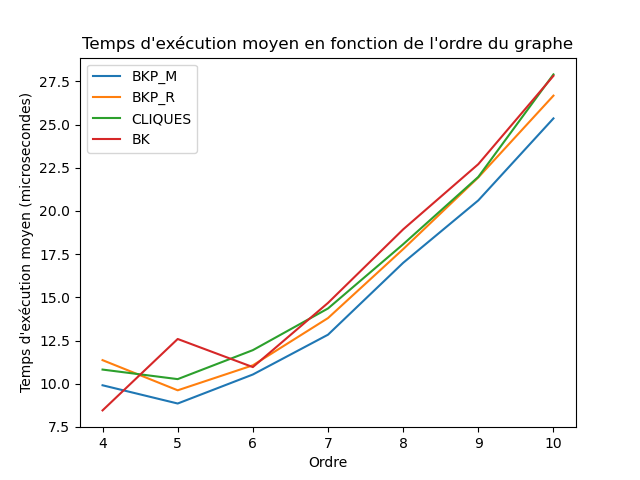
\includegraphics[width=\textwidth]{images/total_plot.png}
        \caption{Temps total moyen pour énumérer toutes les cliques maximales}
        \label{subfig:total_plot}
    \end{subfigure}
    \hfill
    \begin{subfigure}[b]{0.49\textwidth}
        \centering
        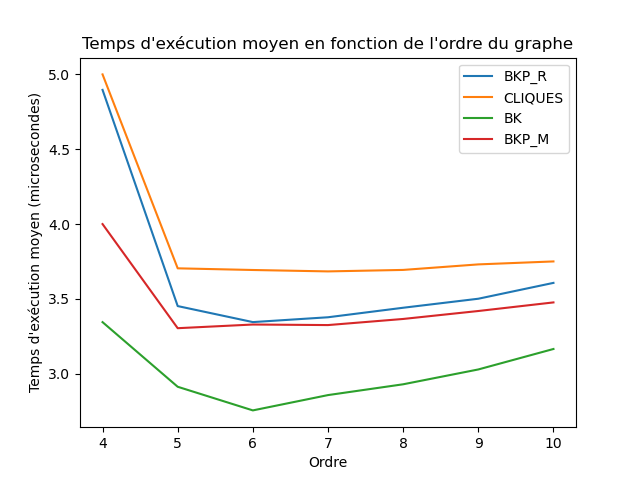
\includegraphics[width=\textwidth]{images/delay_plot.png}
        \caption{Délai moyen pour énumérer une clique maximale}
        \label{subfig:delay_plot}
    \end{subfigure}
    \caption{Résultats des temps d'exécution pour différents algorithmes d'énumération des cliques maximales}
    \label{fig:res1}
\end{figure}

\begin{table}[ht]
  \centering
  \begin{tabular}{|l||l|l|l|l|}
    \hline
    Ordre & BK & BKP\_R & BKP\_M & CLIQUES \\
    \hline
    \hline
    4  & $1.0799^{e-05}$ & $1.6508^{e-05}$ & $1.1213^{e-05}$ & $1.1625^{e-05}$ \\
    5  & $1.2079^{e-05}$ & $1.3219^{e-05}$ & $1.2379^{e-05}$ & $1.3643^{e-05}$ \\
    6  & $1.560e^{e-05}$  & $1.6169^{e-05}$ & $1.5854^{e-05}$  & $1.7883^{e-05}$ \\
    7  & $2.0252^{e-05}$ & $2.0829^{e-05}$ & $1.9958^{e-05}$ & $2.1590^{e-05}$   \\
    8  & $2.5791^{e-05}$ & $2.6625^{e-05}$ & $2.5337^{e-05}$   & $2.7245^{e-05}$ \\
    9  & $3.2806^{e-05}$ & $3.3322^{e-05}$  & $3.189e^{e-05}$  & $3.387e^{e-05}$  \\
    10 & $4.0894^{e-05}$ & $4.1189^{e-05}$ & $3.926e^{e-05}$ & $4.2038^{e-05}$  \\
    \hline
  \end{tabular}
  \caption{Temps d'exécution moyen des algorithmes sur tous les graphes d'ordre 4 à 10}
  \label{table:1}
\end{table}
\begin{table}[ht]
  \centering
  \begin{tabular}{|l||l|l|l|l|}
    \hline
    Ordre & BK & BKP\_R & BKP\_M & CLIQUES \\
    \hline
    \hline
    4  & $3.7588^{e-06}$ & $4.0444^{e-06}$ & $4.5968^{e-06}$ & $5.1999^{e-06}$ \\
    5  & $3.0838^{e-06}$ & $3.5742^{e-06}$ & $3.7282^{e-06}$ & $3.9874^{e-06}$ \\
    6  & $2.8786^{e-06}$ & $3.4932^{e-06}$ & $3.4684^{e-06}$ & $3.7294^{e-06}$ \\
    7  & $2.8994^{e-06}$ & $3.4047^{e-06}$ & $3.4149^{e-06}$ & $3.7131^{e-06}$   \\
    8  & $3.0013^{e-06}$ & $3.5007^{e-06}$ & $3.4537^{e-06}$ & $3.7050^{e-06}$ \\
    9  & $3.1184^{e-06}$ & $3.5931^{e-06}$ & $3.5112^{e-06}$ & $3.8213^{e-06}$  \\
    10 & $3.2128^{e-06}$ & $3.6631^{e-06}$ & $3.5805e^{e-06}$ & $3.8666^{e-06}$  \\
    \hline
    \end{tabular}
    \caption{Délai moyen pour énumérer une clique maximale}
    \label{table:2}
\end{table}

Nous pouvons constater en regardant le graphique \ref{subfig:total_plot} que, clairement, les différents algorithmes d'énumération de cliques présentés suivent bien une complexité en temps exponetiel par rapport à l'ordre du graphe.

De plus, le graphique \ref{subfig:delay_plot} nous montre un temps relativement constant entre l'énumération de chaque clique. Nous pouvons observé un temps moyen pour énumérer les cliques maximales plus élevé pour les graphes d'ordre 4.

En observant les temps obtenu pour les différents algorithmes, nous constatons que \texttt{CLIQUEs} semble se comporter un peu mieux de manière générale.

L'analyse de ces résultats est cohérente avec les discussions théoriques présentées dans l'article \cite{CONTE20221}. L'efficacité des différents algorithmes dépend fortement de leurs approches spécifiques pour traiter les graphes, et la sélection de l'algorithme optimal peut varier en fonction des caractéristiques spécifiques du graphe à traiter.

Afin d'étayer ce dernier propos, nous allons présenter les mêmes tests mais en nous intéressant à des types de graphes particuliers :
\begin{itemize}
  \item Les graphes complets
  \item Les graphes vides
  \item Les graphes de Moon-Moser
\end{itemize}
Pour rappel, les graphes complets d'ordre \emph{n} n'ont qu'une et une seule clique maximales de taille \emph{n}, les graphes vides d'ordre \emph{n} possèdent \emph{n} cliques maximales de taille 1 et enfin, les graphes de Moon-Moser possèdent \(3^{n/3}\) cliques maximales (voir section \ref{subsec:graphes}).

La méthode de test reste la même. L'algorithme sans pivot \texttt{BK} a néanmoins dû être retiré des tests car celui-ci prenait trop de temps d'exécution.

\begin{figure}[ht]
  \centering
  \begin{subfigure}[b]{0.42\textwidth}
    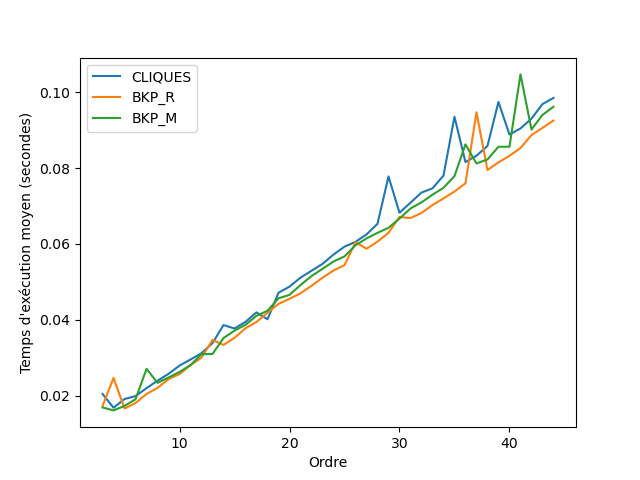
\includegraphics[width=\textwidth]{images/total_pivot_empty_plot.png}
    \caption{Graphes vides}
    \label{subfig:total_empty}
  \end{subfigure}
  \begin{subfigure}[b]{0.42\textwidth}
    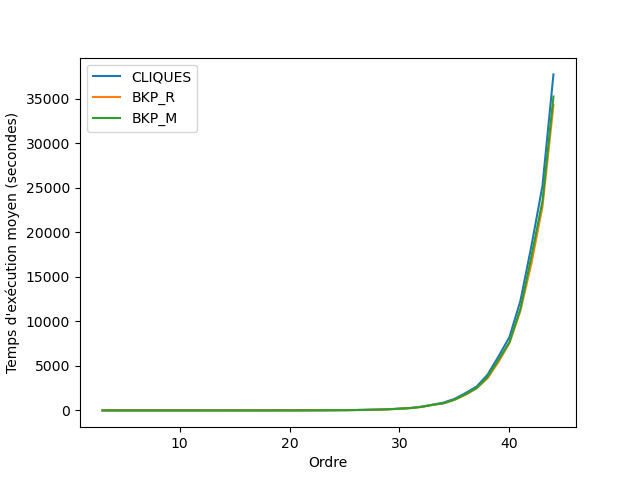
\includegraphics[width=\textwidth]{images/total_pivot_turan_plot.png}
    \caption{Moon-Moser}
    \label{subfig:total_turan}
  \end{subfigure}
  \begin{subfigure}[b]{0.42\textwidth}
    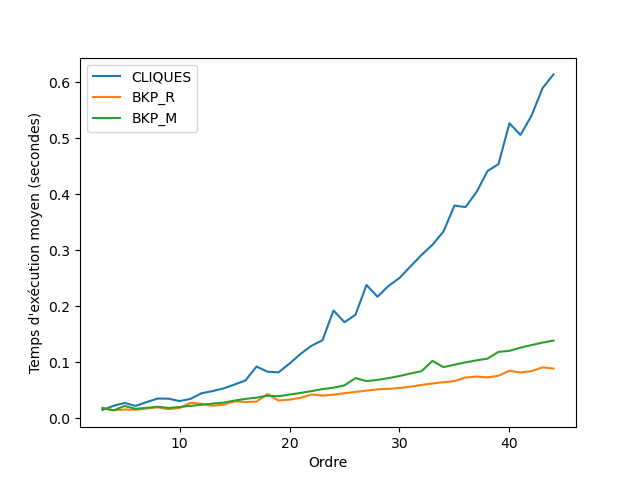
\includegraphics[width=\textwidth]{images/total_pivot_complete_plot.png}
    \caption{Graphes complets}
    \label{subfig:total_complete}
  \end{subfigure}
  \caption{Temps d'exécution total pour énumérer toutes les cliques maximales}
  \label{fig:special_total}
\end{figure}

Tout d'abord, nous pouvons observer qu'en effet, les différents algorithmes présentés ont bien une complexité dans le pire des cas en \(0(3^{n/3})\), cela se voit distinctement sur le graphique \ref{subfig:total_turan} correspondant aux graphes de Moon-Moser, les graphes avec le plus de cliques maximales possible. Pour ce qui est des graphes vides (\ref{subfig:total_empty}), nous avons quelque chose de très linéaire, ce qui s'explique probablement par le fait que, vu que chaque noeud est isolé, énumérer chaque clique maximale consiste à énumérer chaque noeud du graphe. Aucune exploration n'est nécessaire. Quelque chose de curieux se passe avec les graphes complets. En effet, on voit cairement sur la Figure \ref{subfig:total_complete} que l'algorithme CLIQUES a des performances bien médiocre comparé aux autres et que la version de BK avec un pivot aléatoire est sensiblement la meilleur. Cela s'explique par la façon dont le pivot est calculé. Pour rappel, voici comment est trouvé le pivot pour CLIQUES et BKP\_M :

\begin{algorithm}[H]
  \begin{algorithmic}[1]
    \Procedure{CLIQUES}{}
        \State $u \gets$ un noeud de $SUBG$ qui maximise $|CAND \cap N(u)|$
    \EndProcedure
  \end{algorithmic}
  \label{fig:pivot_cliques}
  \begin{algorithmic}[1]
    \Procedure{BKP\_M}{}
        \State $u \gets$ un noeud de $SUBG$ qui maximise $|N(u)|$
    \EndProcedure
  \end{algorithmic}
  \caption{CLIQUES vs BKP\_M}
  \label{fig:pivot_bkp_m}
\end{algorithm}

Étant donné qu'un graphe complet d'ordre \emph{n} ne contient qu'une et une seule clique maximale, l'ensemble des candidats et l'ensemble des voisins d'un noeud sont les mêmes et sont de taille \emph{n}.
Dans le cas de CLIQUES, pour trouver un noeud pivot, nous devons itérer sur tous les noeuds de \texttt{SUBG} (taille \emph{n}) et réaliser l'intersection entre \texttt{CAND} et \texttt{N(u)} or, vu que ces 2 ensembles sont également de taille \emph{n}, cela se fait en \(O(n)\). Nous avons donc un pire des cas atteint de façon systématique qui est en \(n * O(n) = O(n^2)\).
Dans le cas de l'algorithme \texttt{BKP\_M} pour trouver le noeud de degré maximum, il suffit d'itérer sur tout les noeuds et récupérer la longueur de sa liste de voisins, ce qui nous donne une complexité de \(n * O(1) = O(n)\).
Pour le pivot aléatoire, l'opération consistant à choisir un noeud pivot se fait trivialement en temps constant (\(O(1)\)).
Cela explique clairement pourquoi CLIQUES performe moins bien dans ce cas-ci et pourquoi la version avec un pivot aléatoire de BK est la plus efficace, le choix du pivot dans un graphe complet n'ayant pas d'importance étant donné que n'importe quel pivot mènera à la seule clique maximale existante.

Ce constat est aussi valable pour le délai (voir Figure \ref{fig:special_delay}).
\begin{figure}[ht]
  \centering
  \begin{subfigure}[b]{0.42\textwidth}
    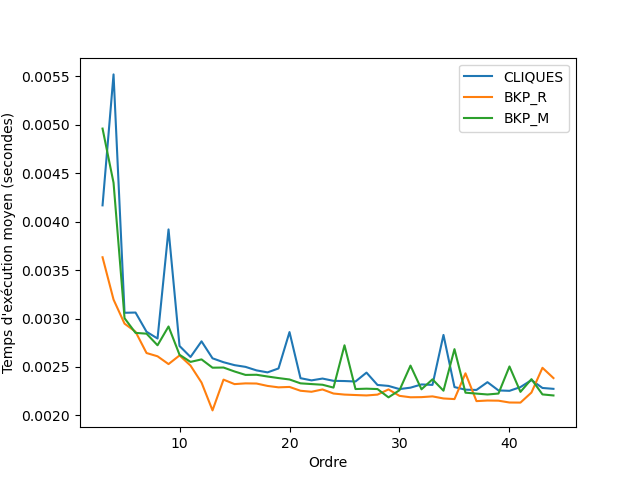
\includegraphics[width=\textwidth]{images/delay_pivot_empty_plot.png}
    \caption{Graphes vides}
    \label{subfig:delay_empty}
  \end{subfigure}
  \begin{subfigure}[b]{0.42\textwidth}
    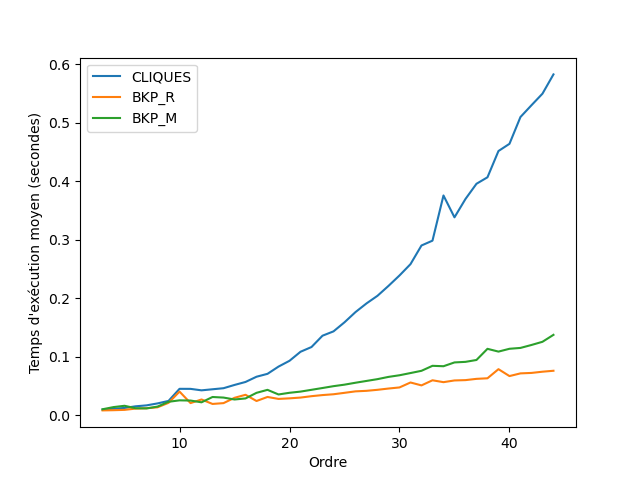
\includegraphics[width=\textwidth]{images/delay_pivot_turan_plot.png}
    \caption{Moon-Moser}
    \label{subfig:delay_turan}
  \end{subfigure}
  \begin{subfigure}[b]{0.42\textwidth}
    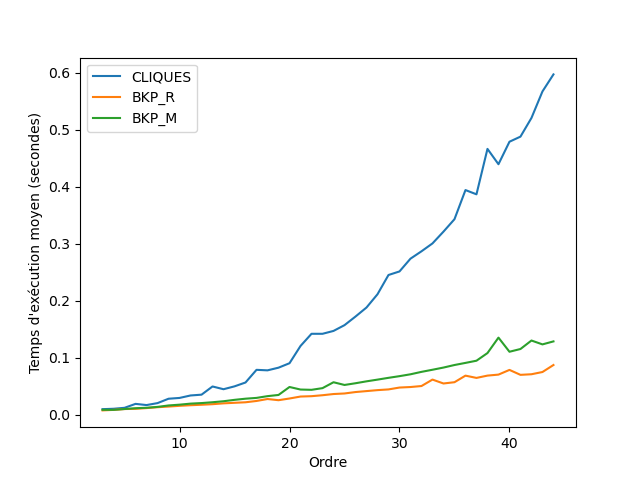
\includegraphics[width=\textwidth]{images/delay_pivot_complete_plot.png}
    \caption{Graphes complets}
    \label{subfig:delay_complete}
  \end{subfigure}
  \caption{Délai entre chaque énumération de clique maximale}
  \label{fig:special_delay}
\end{figure}

Observons maintenant sur ces catégories de graphes ce qu'il en est du délai nécessaire pour trouver la prochaine clique maximale. Dans les deux cas, nous avons bien un délai qui semble polynomial en fonction du nombre de cliques ce qui est rassurant. Toutefois, il est important de souligner que l'algorithme \texttt{CLIQUES} semble moins efficace et mette plus de temps que les autres. Cela va à l'encontre des résultats attendus et est probablement dû à l'implémentation réalisée. En effet, trouver le noeud pivot nécessite, pour chaque noeud de \texttt{SUBG}, de calculer \(\texttt{CAND} \cap N(u)\) afin de trouver le noeud qui maximise cette propriété, ce qui a un coût plus grand que de trouver le noeud de degré supérieur, cela même ayant un coût plus grand que de tirer un noeud au hasard.\footnote{Vous trouverez les tableaux avec les données précises en annexes pour tous les graphes spéciaux.}

\subsubsection*{Comparaison avec \emph{Rust}}

L'une des revendications de ce projet est que, bien implémenté, un algorithme équivalent en \emph{Rust} devrait être plus performant que son homonyme écrit en \emph{Python}. Bien évidemment, il va de soit que cela dépend de la qualité de l'implémentation.

\begin{figure}[ht]
  \centering
  \begin{subfigure}[b]{0.45\textwidth}
    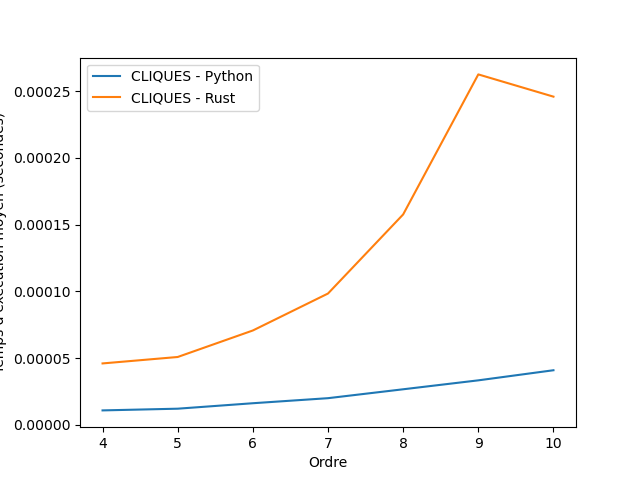
\includegraphics[width=\textwidth]{images/total_pyrust_CLIQUES_plot.png}
  \caption{CLIQUES}%
  \label{subfig:pr_cliques}
  \end{subfigure}
  \begin{subfigure}[b]{0.45\textwidth}
    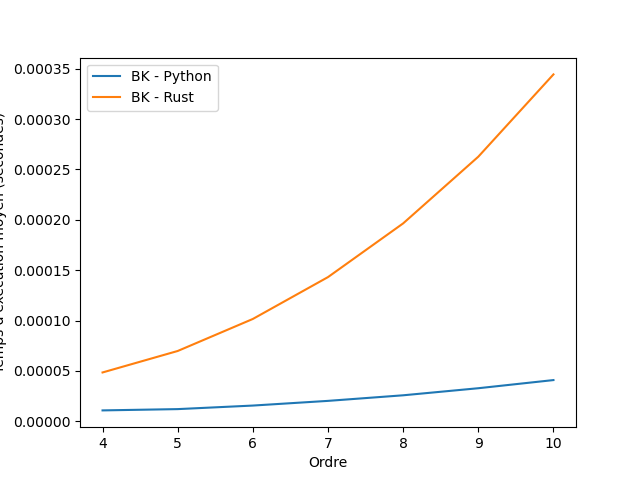
\includegraphics[width=\textwidth]{images/total_pyrust_BK_plot.png}
  \caption{Bron-Kerbosch}%
  \label{subfig:pr_bk}
  \end{subfigure}
  \begin{subfigure}[b]{0.45\textwidth}
    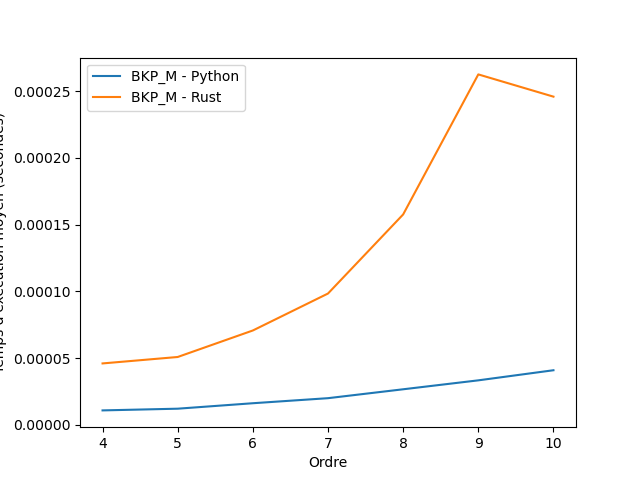
\includegraphics[width=\textwidth]{images/total_pyrust_BKP_M_plot.png}
  \caption{BKP\_M}%
  \label{subfig:pr_bkp_m}
  \end{subfigure}
  \begin{subfigure}[b]{0.45\textwidth}
    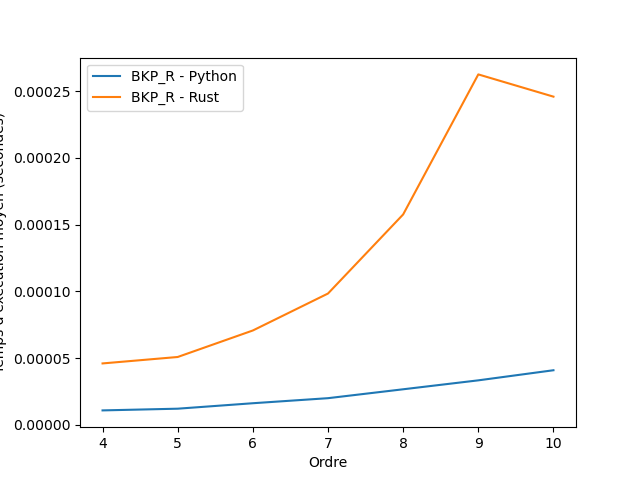
\includegraphics[width=\textwidth]{images/total_pyrust_BKP_R_plot.png}
  \caption{BKP\_R}%
  \label{subfig:pr_bkp_r}
  \end{subfigure}
  \caption{Comparaison des différents algorithmes en \emph{Python} et \emph{Rust}}%
  \label{fig:pvr}
\end{figure}

\begin{figure}[ht]
  \centering
  \begin{subfigure}[b]{0.32\textwidth}
    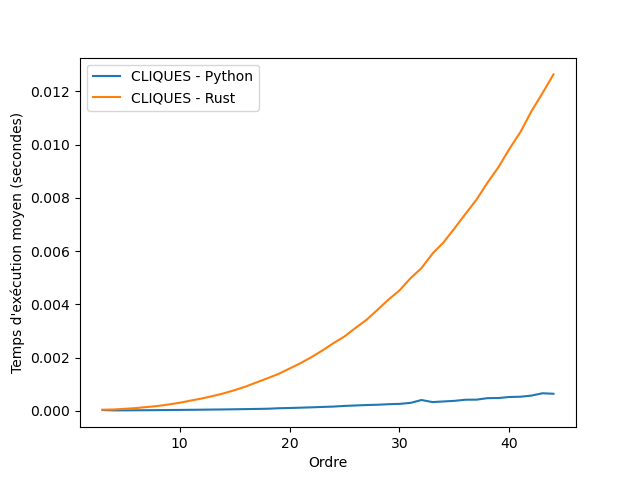
\includegraphics[width=\textwidth]{images/total_CLIQUES_pyrust_pivot_complete_plot.png}
  \caption{Graphes complets}%
  \label{subfig:pr_cliques_complete}
  \end{subfigure}
  \begin{subfigure}[b]{0.32\textwidth}
    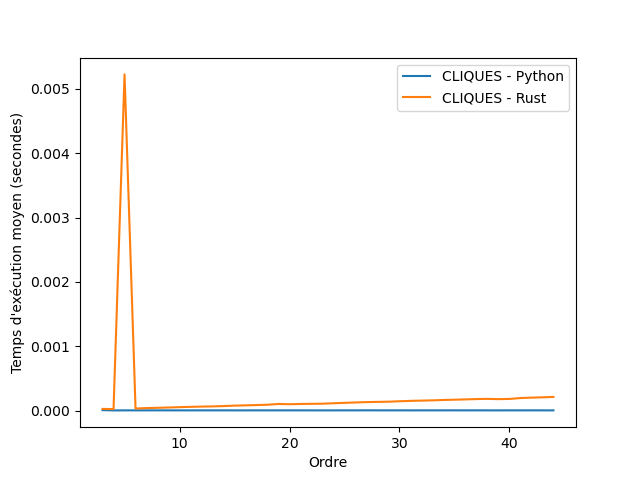
\includegraphics[width=\textwidth]{images/total_CLIQUES_pyrust_pivot_empty_plot.png}
  \caption{Graphes vides}%
  \label{subfig:pr_cliques_empty}
  \end{subfigure}
  \begin{subfigure}[b]{0.32\textwidth}
    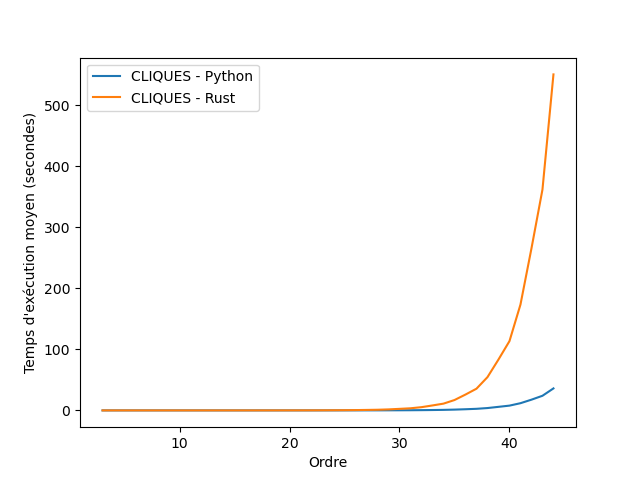
\includegraphics[width=\textwidth]{images/total_CLIQUES_pyrust_pivot_turan_plot.png}
  \caption{Moon-Moser}%
  \label{subfig:pr_cliques_turan}
  \end{subfigure}
  \caption{Comparaison de CLIQUES en \emph{Python} et \emph{Rust} sur des graphes spéciaux}%
  \label{fig:pvr_cliques}
\end{figure}

Étonnamment, nous avons l'opposé du résultat attendu. En effet, on peut clairement voir que les versions \emph{Python} sont constamment meilleures que leurs équivalentes en \emph{Rust}. Ce résultat semble surprenant mais comme mentionné précédemment, le \emph{Rust} est un langage de plus bas niveau et plus complexe dans son fonctionnement que \emph{Python} et cela est plus que certainement dû à une mauvaise implémentation. Au vu des résultats obtenus, une révision des versions \emph{Rust} fut effectuée et ces lignes de code \emph{Rust} (présentent dans chaque algorithmes) ont retenu notre attention :

\begin{figure}[ht]
  \begin{lstlisting}[language=Rust]
let subg_p: HashSet<u32> = subg.intersection(&p_neighbors).cloned().collect();
let cand_p: HashSet<u32> = cand.intersection(&p_neighbors).cloned().collect();

cliques(&mut subg_p.clone(), &mut cand_p.clone(), q, g, result, delay);
  \end{lstlisting}
  \caption{Extrait du code \emph{Rust} de CLIQUES}
  \label{fig:bad_rust}
\end{figure}


Assez étrangement malgré le calcul de l'intersection entre \texttt{SUBG / CAND} et \texttt{N(p)} on peut voir que nous effectuons une nouvelle copie de ces ensembles nouvellement calculés lors de l'appel récursif. Si l'on retire le \texttt{.clone()} dans l'appel récursif, le compilateur se plaint qu'il ne peut pas emprunter les-dits valeurs\footnote{Voir la documentation officielle de \emph{Rust} pour comprendre le principe d'emprunt \href{https://doc.rust-lang.org/stable/book/ch04-00-understanding-ownership.html}{ici}} de façon mutable. Cela se fixe facilement en copiant les ensembles, ainsi nous obtenons notre propre copie que nous pouvons emprunter de façon mutable, malheureusement cela introduit une copie inutile pour ces deux ensembles.
Après révision du code il s'avère que pour éviter ces copies, il suffit de déclarer \texttt{subg\_p} et \texttt{cand\_p} comme des variables mutables avec le mot clé \texttt{mut}. Désormais il est possible de passer les ensembles à l'appel récursif et celui-ci peut les emprunter sans soucis.

Certe l'éliminations de ces \texttt{.clone()} inutile est une bonne nouvelle mais comme mentionné dans la section sur l'implémentation en \emph{Rust} (\ref{subsec:rust}), d'autres sont présents. Notamment au calcul de \texttt{subg\_p} et \texttt{cand\_p} mais aussi de la boucle lors du calcul de \[ CAND - N(u) \]. Après des recherchents plus approfondies il se trouve que que la fonction \texttt{.copied()} existe et peut-être utilisée en lieu et place de \texttt{.cloned()}. cette fonction peut s'avérer plus performante dans certain cas (surtout avec des types primitifs). Extrait de la documentation officielle de \emph{Rust} à propos de \texttt{Clone} : \textit{\guillemotleft Differs from Copy in that Copy is implicit and an inexpensive bit-wise copy, while Clone is always explicit and may or may not be expensive. \guillemotright}

Tout cela a mené à une amélioration des performances de -+ 20\%, ce qui est un début mais cela reste loin du résultat attendu. \emph{Python} reste toujours meilleur que \emph{Rust}. Après discussion avec des personnes plus familière avec le langage, il est apparu que le soucis de performance ne venait pas du code mais de la façon dont celui-ci est exécuté. Jusqu'à présent, nous utilisions la commande \texttt{cargo run}, or, cette commande correspond au mode \emph{debug} de \emph{Rust} et compile le code mais sans optimisations. Pour profiter pleinement de la puissance du langage, il est recommandé d'utiliser la commande \texttt{cargo run --release}\footnote{Plus d'information : \url{https://doc.rust-lang.org/stable/book/ch01-03-hello-cargo.html}}.


\begin{figure}[ht]
  \centering
  \begin{subfigure}[b]{0.24\textwidth}
    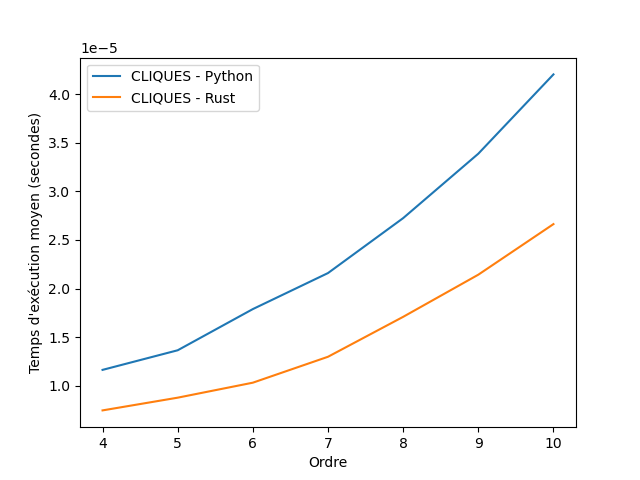
\includegraphics[width=\textwidth]{images/total_new_pyrust_CLIQUES_plot.png}
  \caption{CLIQUES}%
  \label{subfig:pr2_cliques}
  \end{subfigure}
  \begin{subfigure}[b]{0.24\textwidth}
    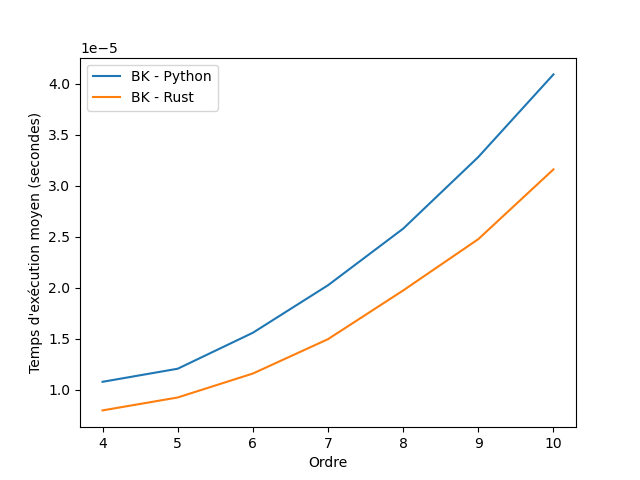
\includegraphics[width=\textwidth]{images/total_new_pyrust_BK_plot.png}
  \caption{Bron-Kerbosch}%
  \label{subfig:pr2_bk}
  \end{subfigure}
  \begin{subfigure}[b]{0.24\textwidth}
    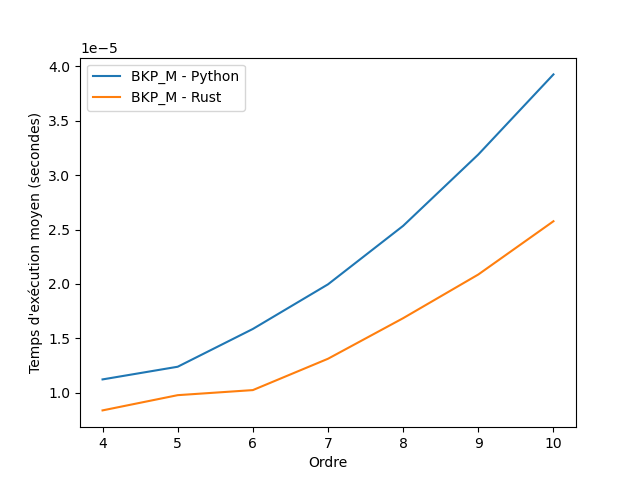
\includegraphics[width=\textwidth]{images/total_new_pyrust_BKP_M_plot.png}
  \caption{BKP\_M}%
  \label{subfig:pr2_bkp_m}
  \end{subfigure}
  \begin{subfigure}[b]{0.24\textwidth}
    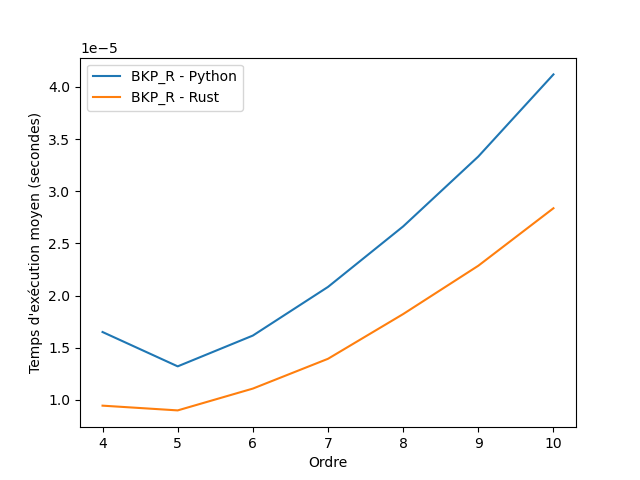
\includegraphics[width=\textwidth]{images/total_new_pyrust_BKP_R_plot.png}
  \caption{BKP\_R}%
  \label{subfig:pr2_bkp_r}
  \end{subfigure}
  \caption{Comparaison des différents algorithmes en \emph{Python} et \emph{Rust}, temps total moyen}%
  \label{fig:pvr2}
\end{figure}

\begin{figure}[ht]
  \centering
  \begin{subfigure}[b]{0.24\textwidth}
    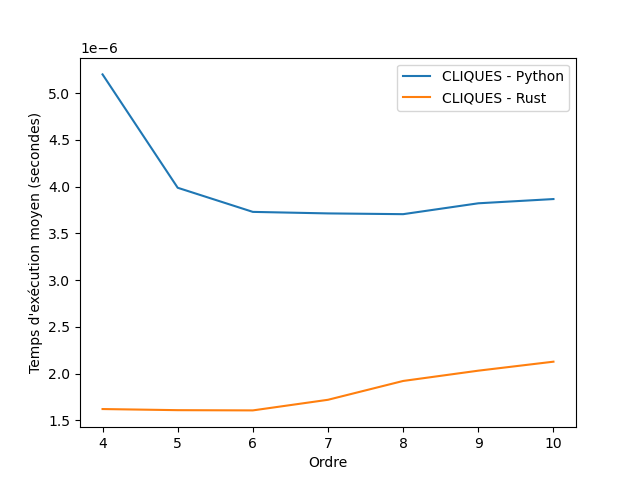
\includegraphics[width=\textwidth]{images/delay_new_pyrust_CLIQUES_plot.png}
  \caption{CLIQUES}%
  \label{subfig:pr2_delay_cliques}
  \end{subfigure}
  \begin{subfigure}[b]{0.24\textwidth}
    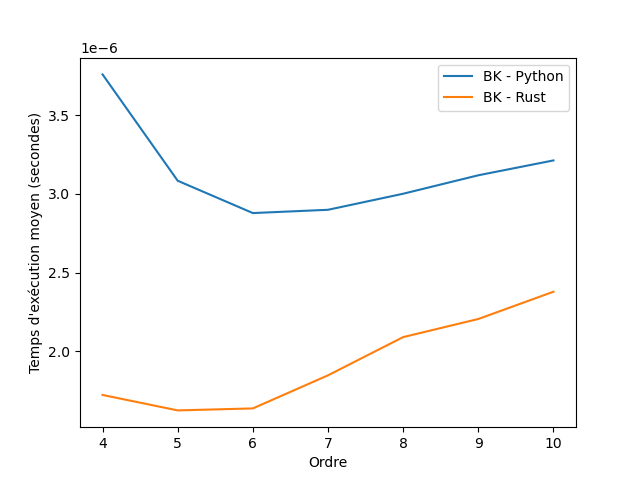
\includegraphics[width=\textwidth]{images/delay_new_pyrust_BK_plot.png}
  \caption{Bron-Kerbosch}%
  \label{subfig:pr2_delay_bk}
  \end{subfigure}
  \begin{subfigure}[b]{0.24\textwidth}
    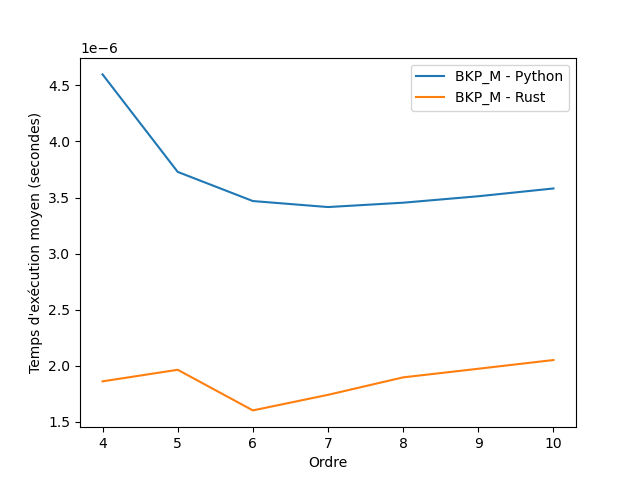
\includegraphics[width=\textwidth]{images/delay_new_pyrust_BKP_M_plot.png}
  \caption{BKP\_M}%
  \label{subfig:pr2_delay_bkp_m}
  \end{subfigure}
  \begin{subfigure}[b]{0.24\textwidth}
    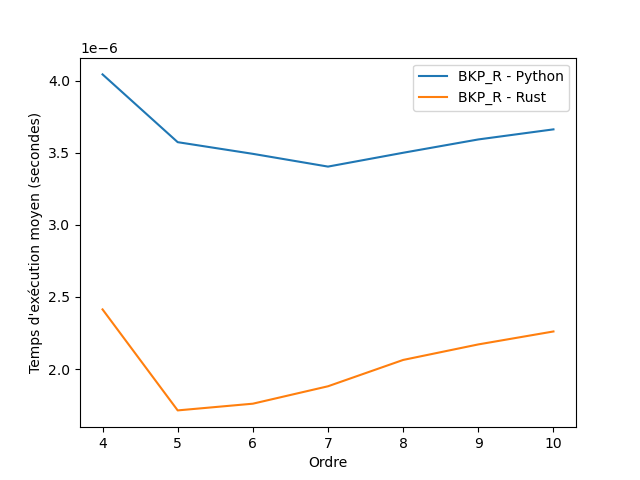
\includegraphics[width=\textwidth]{images/delay_new_pyrust_BKP_R_plot.png}
  \caption{BKP\_R}%
  \label{subfig:pr2_delay_bkp_r}
  \end{subfigure}
  \caption{Comparaison des différents algorithmes en \emph{Python} et \emph{Rust}, délais moyen}%
  \label{fig:pvr2_delay}
\end{figure}

En utilisant la commande indiquée nous avons désormais des résultats cohérents. Les Figures \ref{fig:pvr2} et \ref{fig:pvr2_delay} montrent bien que de manière générale \emph{Rust} est plus efficace que \emph{Python}, ce qui était un résultat attendu. Ce résultat est encourageant et montre l'importance du choix du langage pour des tâches complexes et prenant du temps.

La Figure \ref{fig:pvr2_all} compare le temps total pour énumérer toutes les cliques sur des graphes spéciaux. Nous pouvons constater des résultats beaucoup plus mitigés. En effet, pour les graphes complets et de Moon-Moser nous n'observons pas de meilleur temps d'exécution, bien au contraire, dans le cas des graphes vides nous avons même des performances bien pire et ce, peu importe l'algorithme utilisé. Cela est dû au fait que le code \emph{Rust} fait plus de travail lors de la création de la boucle permettant d'itérer sur \(CAND - N(u)\).

\begin{figure}[h!]
  \centering
  \begin{subfigure}[b]{0.32\textwidth}
    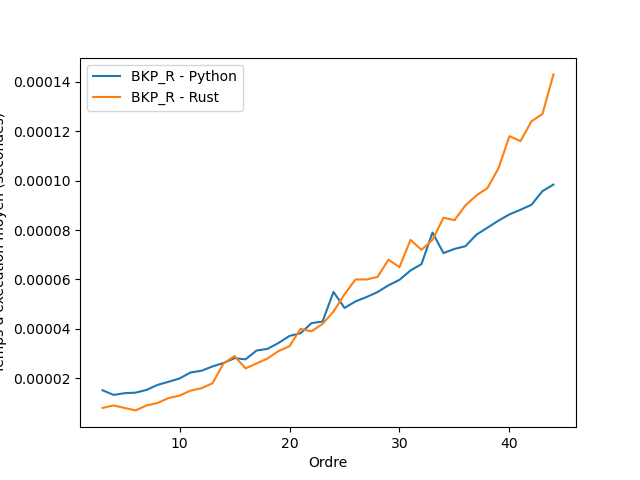
\includegraphics[width=\textwidth]{images/total_BKP_R_new_pyrust_pivot_complete_plot.png}
  \caption{Graphes complets}%
  \label{subfig:pr2_BKP_R_complete}
  \end{subfigure}
  \begin{subfigure}[b]{0.32\textwidth}
    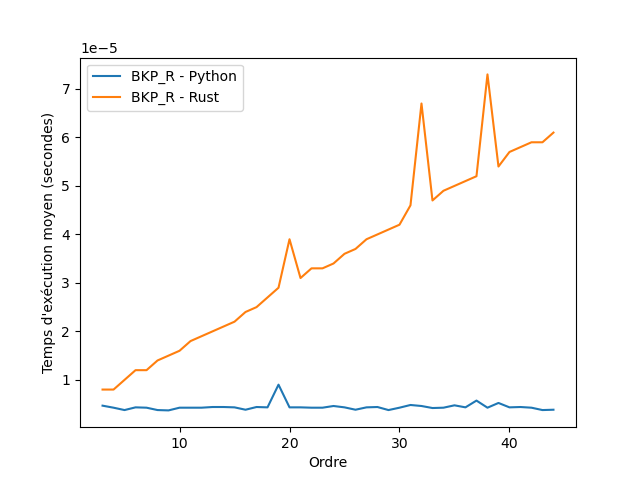
\includegraphics[width=\textwidth]{images/total_BKP_R_new_pyrust_pivot_empty_plot.png}
  \caption{Graphes vides}%
  \label{subfig:pr2_BKP_R_empty}
  \end{subfigure}
  \begin{subfigure}[b]{0.32\textwidth}
    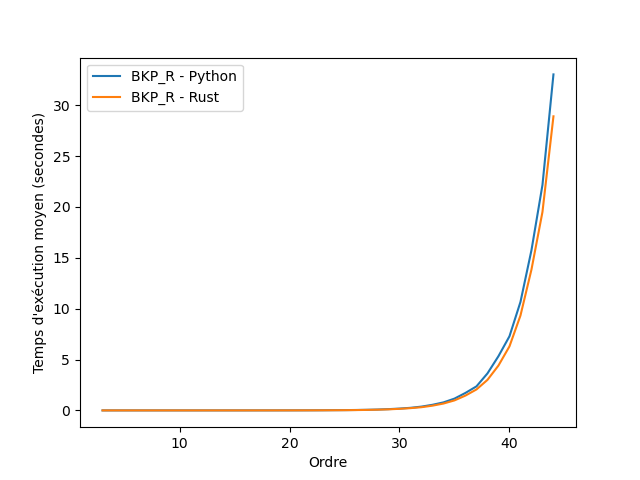
\includegraphics[width=\textwidth]{images/total_BKP_R_new_pyrust_pivot_turan_plot.png}
  \caption{Moon-Moser}%
  \label{subfig:pr2_BKP_R_turan}
  \end{subfigure}
  \begin{subfigure}[b]{0.32\textwidth}
    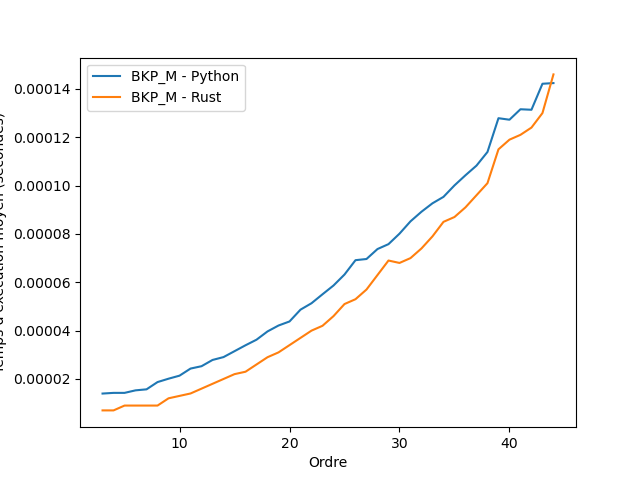
\includegraphics[width=\textwidth]{images/total_BKP_M_new_pyrust_pivot_complete_plot.png}
  \caption{Graphes complets}%
  \label{subfig:pr2_BKP_M_complete}
  \end{subfigure}
  \begin{subfigure}[b]{0.32\textwidth}
    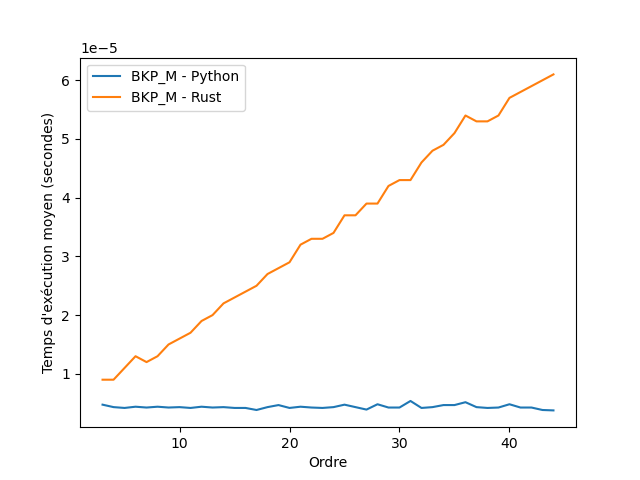
\includegraphics[width=\textwidth]{images/total_BKP_M_new_pyrust_pivot_empty_plot.png}
  \caption{Graphes vides}%
  \label{subfig:pr2_BKP_M_empty}
  \end{subfigure}
  \begin{subfigure}[b]{0.32\textwidth}
    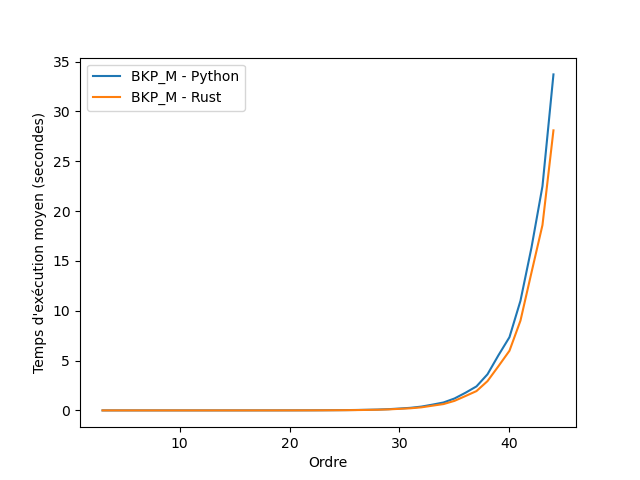
\includegraphics[width=\textwidth]{images/total_BKP_M_new_pyrust_pivot_turan_plot.png}
  \caption{Moon-Moser}%
  \label{subfig:pr2_BKP_M_turan}
  \end{subfigure}
  \begin{subfigure}[b]{0.32\textwidth}
    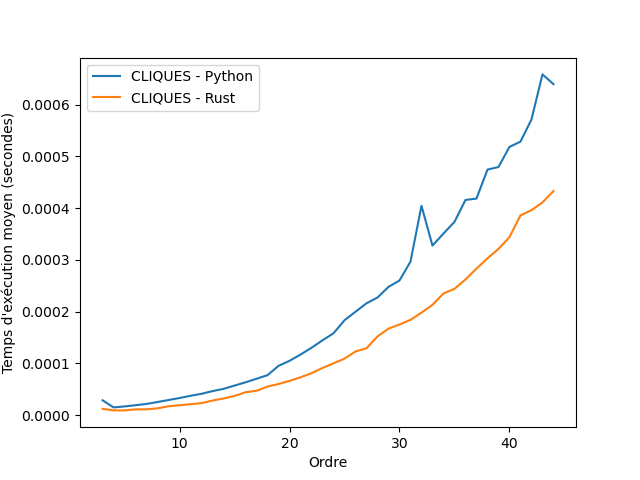
\includegraphics[width=\textwidth]{images/total_CLIQUES_new_pyrust_pivot_complete_plot.png}
  \caption{Graphes complets}%
  \label{subfig:pr2_cliques_complete}
  \end{subfigure}
  \begin{subfigure}[b]{0.32\textwidth}
    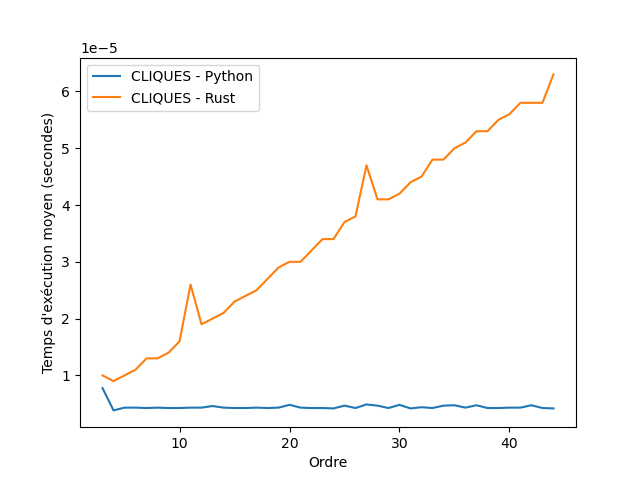
\includegraphics[width=\textwidth]{images/total_CLIQUES_new_pyrust_pivot_empty_plot.png}
  \caption{Graphes vides}%
  \label{subfig:pr2_cliques_empty}
  \end{subfigure}
  \begin{subfigure}[b]{0.32\textwidth}
    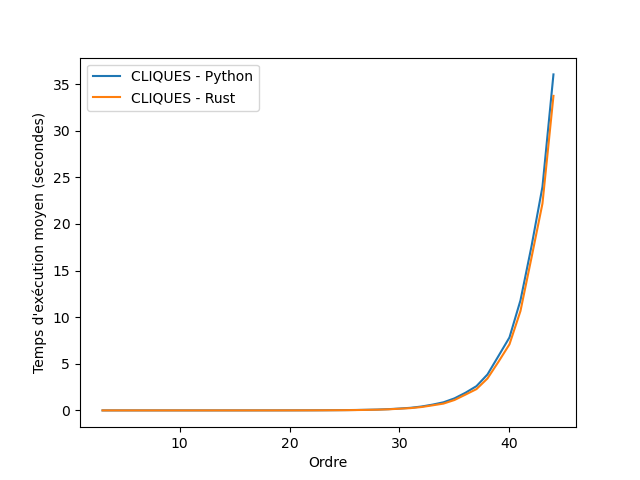
\includegraphics[width=\textwidth]{images/total_CLIQUES_new_pyrust_pivot_turan_plot.png}
  \caption{Moon-Moser}%
  \label{subfig:pr2_cliques_turan}
  \end{subfigure}
  \caption{Comparaison entre \emph{Python} et \emph{Rust} sur des graphes spéciaux}%
  \label{fig:pvr2_all}
\end{figure}
\begin{table}
  \centering
  \begin{tabular}{|l||l|l|l|l|}
    \hline
    Ordre & BK & BKP\_R & BKP\_M & CLIQUES \\
    \hline
    \hline
    4 & $\downarrow-35.9^{\%}$ & $\downarrow-42.7^{\%}$ & $\downarrow-25.4^{\%}$ & $\downarrow-25.9^{\%}$ \\
    5 & $\downarrow-35.8^{\%}$ & $\downarrow-31.9^{\%}$ & $\downarrow-21.1^{\%}$ & $\downarrow-23.3^{\%}$ \\
    6 & $\downarrow-42.4^{\%}$ & $\downarrow-31.4^{\%}$ & $\downarrow-35.5^{\%}$ & $\downarrow-25.6^{\%}$ \\
    7 & $\downarrow-39.9^{\%}$ & $\downarrow-33.1^{\%}$ & $\downarrow-34.3^{\%}$ & $\downarrow-26.1^{\%}$ \\
    8 & $\downarrow-37.3^{\%}$ & $\downarrow-31.5^{\%}$ & $\downarrow-33.5^{\%}$ & $\downarrow-23.5^{\%}$ \\
    9 & $\downarrow-36.8^{\%}$ & $\downarrow-31.4^{\%}$ & $\downarrow-34.6^{\%}$ & $\downarrow-24.5^{\%}$ \\
    10 & $\downarrow-36.7^{\%}$ & $\downarrow-31.1^{\%}$ & $\downarrow-34.4^{\%}$ & $\downarrow-22.7^{\%}$ \\
    \hline
  \end{tabular}
  \caption{Gain de temps moyen d'exécution de \emph{Rust} par rapport à \emph{Python} en pourcentage (Plus bas signifie de meilleures performances)}
  \label{table:rust_total}
\end{table}

De manière générale, \emph{Rust} reste plus performant même s'il est recommandé malgré des performances médiocre sur des graphes vides et équivalentes sur des graphes complets et de Moon-Moser. Également, il est probable qu'il soit possible d'améliorer les implémentations \emph{Rust} en utilisant une autre approche plus propice au langage que les \emph{HashSet} qui, certes, marchent bien en \emph{Python} mais induisent des copies superflues en \emph{Rust}.

\newpage
\section{Conclusion}

Dans ce rapport, nous avons présenté les notions nécessaires à la compréhension du problème d'énumération de toute les cliques maximales d'un graphe simple et expliqué celui-ci. Nous avons discuté de la difficulté de ce problème et présenté plusieurs algorithmes permettant de le résoudre de façon exacte. Ces algorithmes sont tous basés sur l'algorithme de Bron et Kerbosch \cite{bron1973algorithm}. Ainsi nous avons présenté les quatres algorithmes étudiés dans ce rapport : CLIQUES, Bron-Kerbosch et deux variante de ce dernier. L'objectif était de mettre en évidence le gain de performance obtenu par le choix d'un \emph{bon} noeud pivot afin de couper dans l'exploration des cliques maximales. De façon a étayer ces propos, une implémentation en \emph{Python} de ces algorithmes a été réalisée, permettant une évaluation expérimentale de ceux-ci.

Dans un premier temps, les résultats obtenus ont confirmé les complexités de ces derniers et mis en évidence qu'un bon pivot peu améliorer sensiblement les choses.

Afin d'aller plus loin nous avons pris des graphes spéciaux, décrits au préalable, afin de mettre en lumière des différences de performances plus significatives entre les quatres algorithmes. Nous avons donc testé sur des graphes vides, complet et de Moon-Moser afin de voir si ces graphes montraient des tendances différentes. Nous avons pu constater que c'est le cas : CLIQUES se comporte mal sur les graphes complets à cause de la façon dont il caclule son pivot. En essayant de tester nos implémentations sur de grands graphes tirés de cas réel, nous avons pu mettre en évidence les limites techniques de celles-ci étant donné que le matériel utilisé n'était pas suffisant pour gérer des graphes de cette taille. Une façon d'améliorer ce point pourrait être d'utiliser les générateurs de \emph{Python} et de réécrire les algorithmes pour les utiliser directement et ainsi permettre leur utilisation sur de plus grands graphes.

Dans un second temps, nous souhaitions montrer l'importance du choix du langage de programmation pour ce genre d'algorithme et des gains de performances qui peuvent s'en suivre. Ainsi une version en \emph{Rust}, langage de bas niveau, a été réalisée avec le postulat que le \emph{Rust} serait plus efficace. Nous avons constaté la difficulté de traduire d'un langage de haut niveau à un autre langage de programmation de bas niveau, rendant de ce fait toute implémentation plus enclin à avoir des défauts d'optimisation, ceci étant dû à une moins bonne maitrise de ce dernier. Il est clair qu'une meilleure maitrise du langage permettrait d'obtenir de bien meilleurs résultats. De surcroit, nous avons pu constater l'importance de la maitrise d'un langage. Dans le cas de \emph{Rust}, afin de profiter de ses optimisation, il est nécessaire de compiler le code en mode \emph{release}. En finalité \emph{Rust} est plus performant que \emph{Python} même si certains cas montrent le contraire. Une piste pour améliorer cette implémentation serait d'utiliser d'autres structures de données que équivalents à celles utilisées en \emph{Python}.

En conclusion, ce projet m'a permis de comprendre et comparer des algorithmes pointus sur un sujet de recherche actif, de comprendre les défis liés à l'implémentation de ceux-ci et de constater les différences entre les attentes théoriques et les résultats expérimentaux. Également, ce projet m'a permis de me familiariser davantage avec le langage \emph{Rust} et de mieux comprendre des mécanismes que je n'avais encore jamais rencontré. J'ai pu me rendre compte aussi de la difficulté de traduire d'un langage à un autre des algorithmes et de voir qu'il était plus que facile de faire des erreurs menant à une détérioration notable des performances par rapport à ce qui est attendu.

Enfin ce projet m'a permis d'améliorer la qualité de ma rédaction en m'enseignant à mieux vulgariser et illustrer mes propos mais aussi en y apportant une meilleure structure. Il est certain que cela me servira à l'avenir dans mes prochaines productions écrites.

% TODO

\newpage
\bibliographystyle{abbrv}
\bibliography{biblio}

\appendix

\begin{longtable}{|l||l|l|l|l|}
  \hline
  Ordre & Graphe & CLIQUES & BKP\_R & BKP\_M  \endhead
  \hline
  \hline
  \textbf{Ordre} & \textbf{Graphe} & \textbf{CLIQUES} & \textbf{BKP\_R} & \textbf{BKP\_M} \\
  \hline
  \endfirsthead
  \hline
  \textbf{Ordre} & \textbf{Graphe} & \textbf{CLIQUES} & \textbf{BKP\_R} & \textbf{BKP\_M} \\
  \hline
  \endhead
  \hline
  \endfoot
  \hline
  \endlastfoot
  5 & Empty & $4.33e-06$ & $3.77e-06$ & $4.19e-06$ \\
  & Moon-Moser & $2.33e-05$ & $2.34e-05$ & $2.33e-05$ \\
  & Complete & $1.67e-05$ & $1.40e-05$ & $1.42e-05$ \\
  \hline
  6 & Empty & $4.33e-06$ & $4.33e-06$ & $4.40e-06$ \\
  & Moon-Moser & $3.29e-05$ & $2.92e-05$ & $3.00e-05$ \\
  & Complete & $1.90e-05$ & $1.42e-05$ & $1.53e-05$ \\
  \hline
  7 & Empty & $4.26e-06$ & $4.26e-06$ & $4.26e-06$ \\
  & Moon-Moser & $5.58e-05$ & $4.20e-05$ & $4.18e-05$ \\
  & Complete & $2.15e-05$ & $1.53e-05$ & $1.57e-05$ \\
  \hline
  8 & Empty & $4.33e-06$ & $3.77e-06$ & $4.40e-06$ \\
  & Moon-Moser & $6.27e-05$ & $5.84e-05$ & $5.64e-05$ \\
  & Complete & $2.52e-05$ & $1.73e-05$ & $1.87e-05$ \\
  \hline
  9 & Empty & $4.26e-06$ & $3.70e-06$ & $4.26e-06$ \\
  & Moon-Moser & $8.80e-05$ & $7.82e-05$ & $7.93e-05$ \\
  & Complete & $2.91e-05$ & $1.86e-05$ & $2.01e-05$ \\
  \hline
  10 & Empty & $4.26e-06$ & $4.26e-06$ & $4.33e-06$ \\
  & Moon-Moser & $1.22e-04$ & $1.16e-04$ & $1.10e-04$ \\
  & Complete & $3.30e-05$ & $1.99e-05$ & $2.14e-05$ \\
  \hline
  11 & Empty & $4.33e-06$ & $4.26e-06$ & $4.19e-06$ \\
  & Moon-Moser & $1.75e-04$ & $1.59e-04$ & $1.58e-04$ \\
  & Complete & $3.72e-05$ & $2.24e-05$ & $2.43e-05$ \\
  \hline
  12 & Empty & $4.33e-06$ & $4.26e-06$ & $4.40e-06$ \\
  & Moon-Moser & $2.82e-04$ & $2.18e-04$ & $2.35e-04$ \\
  & Complete & $4.11e-05$ & $2.30e-05$ & $2.53e-05$ \\
  \hline
  13 & Empty & $4.61e-06$ & $4.40e-06$ & $4.26e-06$ \\
  & Moon-Moser & $3.51e-04$ & $3.38e-04$ & $3.09e-04$ \\
  & Complete & $4.63e-05$ & $2.48e-05$ & $2.79e-05$ \\
  \hline
  14 & Empty & $4.33e-06$ & $4.40e-06$ & $4.33e-06$ \\
  & Moon-Moser & $4.93e-04$ & $4.63e-04$ & $4.52e-04$ \\
  & Complete & $5.06e-05$ & $2.62e-05$ & $2.91e-05$ \\
  \hline
  15 & Empty & $4.26e-06$ & $4.33e-06$ & $4.19e-06$ \\
  & Moon-Moser & $7.38e-04$ & $6.44e-04$ & $6.72e-04$ \\
  & Complete & $5.70e-05$ & $2.81e-05$ & $3.15e-05$ \\
  \hline
  16 & Empty & $4.26e-06$ & $3.84e-06$ & $4.19e-06$ \\
  & Moon-Moser & $1.02e-03$ & $9.83e-04$ & $9.62e-04$ \\
  & Complete & $6.33e-05$ & $2.77e-05$ & $3.39e-05$ \\
  \hline
  17 & Empty & $4.33e-06$ & $4.40e-06$ & $3.84e-06$ \\
  & Moon-Moser & $1.58e-03$ & $1.42e-03$ & $1.46e-03$ \\
  & Complete & $7.02e-05$ & $3.12e-05$ & $3.62e-05$ \\
  \hline
  18 & Empty & $4.26e-06$ & $4.33e-06$ & $4.33e-06$ \\
  & Moon-Moser & $2.35e-03$ & $2.05e-03$ & $2.16e-03$ \\
  & Complete & $7.71e-05$ & $3.19e-05$ & $3.97e-05$ \\
  \hline
  19 & Empty & $4.33e-06$ & $9.01e-06$ & $4.68e-06$ \\
  & Moon-Moser & $3.21e-03$ & $2.90e-03$ & $2.94e-03$ \\
  & Complete & $9.51e-05$ & $3.43e-05$ & $4.21e-05$ \\
  \hline
  20 & Empty & $4.82e-06$ & $4.33e-06$ & $4.19e-06$ \\
  & Moon-Moser & $4.72e-03$ & $4.26e-03$ & $4.35e-03$ \\
  & Complete & $1.05e-04$ & $3.72e-05$ & $4.38e-05$ \\
  \hline
  21 & Empty & $4.33e-06$ & $4.33e-06$ & $4.40e-06$ \\
  & Moon-Moser & $7.06e-03$ & $6.16e-03$ & $6.48e-03$ \\
  & Complete & $1.17e-04$ & $3.82e-05$ & $4.87e-05$ \\
  \hline
  22 & Empty & $4.26e-06$ & $4.26e-06$ & $4.26e-06$ \\
  & Moon-Moser & $9.55e-03$ & $8.77e-03$ & $8.80e-03$ \\
  & Complete & $1.30e-04$ & $4.23e-05$ & $5.13e-05$ \\
  \hline
  23 & Empty & $4.26e-06$ & $4.26e-06$ & $4.19e-06$ \\
  & Moon-Moser & $1.43e-02$ & $1.29e-02$ & $1.33e-02$ \\
  & Complete & $1.45e-04$ & $4.30e-05$ & $5.50e-05$ \\
  \hline
  24 & Empty & $4.19e-06$ & $4.61e-06$ & $4.33e-06$ \\
  & Moon-Moser & $2.16e-02$ & $2.17e-02$ & $1.99e-02$ \\
  & Complete & $1.58e-04$ & $5.50e-05$ & $5.87e-05$ \\
  \hline
  25 & Empty & $4.68e-06$ & $4.33e-06$ & $4.75e-06$ \\
  & Moon-Moser & $3.03e-02$ & $2.74e-02$ & $2.80e-02$ \\
  & Complete & $1.83e-04$ & $4.85e-05$ & $6.32e-05$ \\
  \hline
  26 & Empty & $4.26e-06$ & $3.84e-06$ & $4.33e-06$ \\
  & Moon-Moser & $4.43e-02$ & $3.98e-02$ & $4.11e-02$ \\
  & Complete & $2.00e-04$ & $5.11e-05$ & $6.91e-05$ \\
  \hline
  27 & Empty & $4.89e-06$ & $4.33e-06$ & $3.91e-06$ \\
  & Moon-Moser & $6.62e-02$ & $5.88e-02$ & $6.19e-02$ \\
  & Complete & $2.16e-04$ & $5.29e-05$ & $6.96e-05$ \\
  \hline
  28 & Empty & $4.68e-06$ & $4.40e-06$ & $4.82e-06$ \\
  & Moon-Moser & $9.01e-02$ & $8.35e-02$ & $8.37e-02$ \\
  & Complete & $2.27e-04$ & $5.49e-05$ & $7.38e-05$ \\
  \hline
  29 & Empty & $4.26e-06$ & $3.77e-06$ & $4.26e-06$ \\
  & Moon-Moser & $1.33e-01$ & $1.24e-01$ & $1.23e-01$ \\
  & Complete & $2.48e-04$ & $5.76e-05$ & $7.58e-05$ \\
  \hline
  30 & Empty & $4.82e-06$ & $4.26e-06$ & $4.26e-06$ \\
  & Moon-Moser & $2.00e-01$ & $1.79e-01$ & $1.87e-01$ \\
  & Complete & $2.60e-04$ & $5.99e-05$ & $8.01e-05$ \\
  \hline
  31 & Empty & $4.19e-06$ & $4.82e-06$ & $5.38e-06$ \\
  & Moon-Moser & $2.78e-01$ & $2.54e-01$ & $2.60e-01$ \\
  & Complete & $2.97e-04$ & $6.36e-05$ & $8.52e-05$ \\
  \hline
  32 & Empty & $4.40e-06$ & $4.61e-06$ & $4.19e-06$ \\
  & Moon-Moser & $4.16e-01$ & $3.73e-01$ & $3.83e-01$ \\
  & Complete & $4.05e-04$ & $6.62e-05$ & $8.92e-05$ \\
  \hline
  33 & Empty & $4.26e-06$ & $4.19e-06$ & $4.33e-06$ \\
  & Moon-Moser & $6.17e-01$ & $5.51e-01$ & $5.79e-01$ \\
  & Complete & $3.28e-04$ & $7.90e-05$ & $9.27e-05$ \\
  \hline
  34 & Empty & $4.68e-06$ & $4.26e-06$ & $4.68e-06$ \\
  & Moon-Moser & $8.68e-01$ & $7.87e-01$ & $7.94e-01$ \\
  & Complete & $3.51e-04$ & $7.07e-05$ & $9.53e-05$ \\
  \hline
  35 & Empty & $4.75e-06$ & $4.75e-06$ & $4.68e-06$ \\
  & Moon-Moser & $1.29e+00$ & $1.16e+00$ & $1.19e+00$ \\
  & Complete & $3.73e-04$ & $7.24e-05$ & $1.00e-04$ \\
  \hline
  36 & Empty & $4.33e-06$ & $4.33e-06$ & $5.17e-06$ \\
  & Moon-Moser & $1.89e+00$ & $1.72e+00$ & $1.77e+00$ \\
  & Complete & $4.16e-04$ & $7.35e-05$ & $1.04e-04$ \\
  \hline
  37 & Empty & $4.75e-06$ & $5.73e-06$ & $4.33e-06$ \\
  & Moon-Moser & $2.60e+00$ & $2.36e+00$ & $2.41e+00$ \\
  & Complete & $4.18e-04$ & $7.82e-05$ & $1.08e-04$ \\
  \hline
  38 & Empty & $4.26e-06$ & $4.26e-06$ & $4.19e-06$ \\
  & Moon-Moser & $3.85e+00$ & $3.64e+00$ & $3.62e+00$ \\
  & Complete & $4.74e-04$ & $8.09e-05$ & $1.14e-04$ \\
  \hline
  39 & Empty & $4.26e-06$ & $5.24e-06$ & $4.26e-06$ \\
  & Moon-Moser & $5.83e+00$ & $5.33e+00$ & $5.54e+00$ \\
  & Complete & $4.79e-04$ & $8.38e-05$ & $1.28e-04$ \\
  \hline
  40 & Empty & $4.33e-06$ & $4.33e-06$ & $4.82e-06$ \\
  & Moon-Moser & $7.83e+00$ & $7.29e+00$ & $7.35e+00$ \\
  & Complete & $5.18e-04$ & $8.63e-05$ & $1.27e-04$ \\
  \hline
  41 & Empty & $4.33e-06$ & $4.40e-06$ & $4.26e-06$ \\
  & Moon-Moser & $1.18e+01$ & $1.07e+01$ & $1.10e+01$ \\
  & Complete & $5.28e-04$ & $8.82e-05$ & $1.32e-04$ \\
  \hline
  42 & Empty & $4.75e-06$ & $4.26e-06$ & $4.26e-06$ \\
  & Moon-Moser & $1.76e+01$ & $1.57e+01$ & $1.63e+01$ \\
  & Complete & $5.71e-04$ & $9.02e-05$ & $1.31e-04$ \\
  \hline
  43 & Empty & $4.26e-06$ & $3.77e-06$ & $3.84e-06$ \\
  & Moon-Moser & $2.40e+01$ & $2.22e+01$ & $2.25e+01$ \\
  & Complete & $6.58e-04$ & $9.58e-05$ & $1.42e-04$ \\
  \hline
  44 & Empty & $4.19e-06$ & $3.84e-06$ & $3.77e-06$ \\
  & Moon-Moser & $3.60e+01$ & $3.30e+01$ & $3.37e+01$ \\
  & Complete & $6.40e-04$ & $9.84e-05$ & $1.42e-04$ \\
  \hline
  \caption{Temps d'exécution total des différents algorithmes sur des graphes spéciaux en \emph{Python}}
\end{longtable}

\begin{longtable}{|l||l|l|l|l|}
  \hline
  \textbf{Ordre} & \textbf{Graphe} & \textbf{CLIQUES} & \textbf{BKP\_R} & \textbf{BKP\_M} \\
  \hline
  \endfirsthead
  \hline
  \textbf{Ordre} & \textbf{Graphe} & \textbf{CLIQUES} & \textbf{BKP\_R} & \textbf{BKP\_M} \\
  \hline
  \endhead
  \hline
  \endfoot
  \hline
  \endlastfoot
  5 & Empty & $2.86e-06$ & $2.86e-06$ & $2.86e-06$ \\
  & Moon-Moser & $3.68e-06$ & $3.10e-06$ & $3.34e-06$ \\
  & Complete & $1.29e-05$ & $9.64e-06$ & $9.50e-06$ \\
  \hline
  6 & Empty & $3.28e-06$ & $2.79e-06$ & $2.79e-06$ \\
  & Moon-Moser & $3.34e-06$ & $3.01e-06$ & $3.10e-06$ \\
  & Complete & $1.56e-05$ & $1.05e-05$ & $1.15e-05$ \\
  \hline
  7 & Empty & $2.86e-06$ & $2.86e-06$ & $2.79e-06$ \\
  & Moon-Moser & $3.59e-06$ & $3.82e-06$ & $2.90e-06$ \\
  & Complete & $2.02e-05$ & $1.24e-05$ & $1.26e-05$ \\
  \hline
  8 & Empty & $2.86e-06$ & $2.86e-06$ & $2.79e-06$ \\
  & Moon-Moser & $3.21e-06$ & $3.07e-06$ & $3.00e-06$ \\
  & Complete & $2.14e-05$ & $1.30e-05$ & $1.47e-05$ \\
  \hline
  9 & Empty & $2.79e-06$ & $2.93e-06$ & $2.86e-06$ \\
  & Moon-Moser & $3.11e-06$ & $2.75e-06$ & $2.84e-06$ \\
  & Complete & $2.49e-05$ & $1.43e-05$ & $1.56e-05$ \\
  \hline
  10 & Empty & $2.79e-06$ & $2.79e-06$ & $2.86e-06$ \\
  & Moon-Moser & $3.21e-06$ & $3.03e-06$ & $2.93e-06$ \\
  & Complete & $2.86e-05$ & $1.76e-05$ & $1.83e-05$ \\
  \hline
  11 & Empty & $2.86e-06$ & $2.86e-06$ & $2.86e-06$ \\
  & Moon-Moser & $3.08e-06$ & $2.85e-06$ & $2.86e-06$ \\
  & Complete & $3.30e-05$ & $1.70e-05$ & $1.92e-05$ \\
  \hline
  12 & Empty & $2.93e-06$ & $2.44e-06$ & $2.93e-06$ \\
  & Moon-Moser & $3.07e-06$ & $2.70e-06$ & $2.75e-06$ \\
  & Complete & $3.52e-05$ & $1.73e-05$ & $2.01e-05$ \\
  \hline
  13 & Empty & $2.93e-06$ & $2.38e-06$ & $2.79e-06$ \\
  & Moon-Moser & $3.31e-06$ & $3.01e-06$ & $2.90e-06$ \\
  & Complete & $5.01e-05$ & $1.91e-05$ & $2.23e-05$ \\
  \hline
  14 & Empty & $2.86e-06$ & $2.86e-06$ & $2.38e-06$ \\
  & Moon-Moser & $3.16e-06$ & $2.81e-06$ & $2.92e-06$ \\
  & Complete & $4.50e-05$ & $1.98e-05$ & $2.40e-05$ \\
  \hline
  15 & Empty & $2.93e-06$ & $2.93e-06$ & $2.86e-06$ \\
  & Moon-Moser & $3.12e-06$ & $2.70e-06$ & $2.84e-06$ \\
  & Complete & $5.01e-05$ & $2.09e-05$ & $4.15e-05$ \\
  \hline
  16 & Empty & $2.86e-06$ & $2.93e-06$ & $2.38e-06$ \\
  & Moon-Moser & $3.15e-06$ & $2.86e-06$ & $2.94e-06$ \\
  & Complete & $5.68e-05$ & $2.28e-05$ & $2.82e-05$ \\
  \hline
  17 & Empty & $2.86e-06$ & $2.86e-06$ & $2.86e-06$ \\
  & Moon-Moser & $3.14e-06$ & $2.75e-06$ & $2.91e-06$ \\
  & Complete & $6.29e-05$ & $2.48e-05$ & $3.02e-05$ \\
  \hline
  18 & Empty & $2.86e-06$ & $2.44e-06$ & $3.28e-06$ \\
  & Moon-Moser & $3.13e-06$ & $2.76e-06$ & $2.90e-06$ \\
  & Complete & $6.97e-05$ & $2.53e-05$ & $3.23e-05$ \\
  \hline
  19 & Empty & $2.79e-06$ & $2.37e-06$ & $2.86e-06$ \\
  & Moon-Moser & $3.23e-06$ & $2.91e-06$ & $2.96e-06$ \\
  & Complete & $7.86e-05$ & $2.77e-05$ & $3.53e-05$ \\
  \hline
  20 & Empty & $2.79e-06$ & $1.95e-06$ & $2.86e-06$ \\
  & Moon-Moser & $3.18e-06$ & $2.85e-06$ & $2.96e-06$ \\
  & Complete & $9.07e-05$ & $2.94e-05$ & $3.82e-05$ \\
  \hline
  21 & Empty & $2.79e-06$ & $2.31e-06$ & $2.86e-06$ \\
  & Moon-Moser & $3.18e-06$ & $2.79e-06$ & $2.95e-06$ \\
  & Complete & $1.09e-04$ & $3.10e-05$ & $4.01e-05$ \\
  \hline
  22 & Empty & $3.28e-06$ & $2.37e-06$ & $2.38e-06$ \\
  & Moon-Moser & $3.25e-06$ & $2.96e-06$ & $2.99e-06$ \\
  & Complete & $1.18e-04$ & $3.31e-05$ & $5.30e-05$ \\
  \hline
  23 & Empty & $2.79e-06$ & $2.86e-06$ & $2.86e-06$ \\
  & Moon-Moser & $3.22e-06$ & $2.91e-06$ & $2.98e-06$ \\
  & Complete & $1.31e-04$ & $3.53e-05$ & $4.64e-05$ \\
  \hline
  24 & Empty & $2.86e-06$ & $2.79e-06$ & $2.44e-06$ \\
  & Moon-Moser & $3.26e-06$ & $2.83e-06$ & $3.08e-06$ \\
  & Complete & $1.45e-04$ & $3.78e-05$ & $4.95e-05$ \\
  \hline
  25 & Empty & $2.44e-06$ & $2.86e-06$ & $2.79e-06$ \\
  & Moon-Moser & $3.42e-06$ & $3.15e-06$ & $3.13e-06$ \\
  & Complete & $1.73e-04$ & $3.90e-05$ & $5.25e-05$ \\
  \hline
  26 & Empty & $2.86e-06$ & $2.30e-06$ & $2.93e-06$ \\
  & Moon-Moser & $3.37e-06$ & $3.03e-06$ & $3.13e-06$ \\
  & Complete & $1.77e-04$ & $4.05e-05$ & $5.57e-05$ \\
  \hline
  27 & Empty & $2.86e-06$ & $2.37e-06$ & $3.21e-06$ \\
  & Moon-Moser & $3.49e-06$ & $3.00e-06$ & $3.13e-06$ \\
  & Complete & $1.93e-04$ & $4.40e-05$ & $5.91e-05$ \\
  \hline
  28 & Empty & $2.86e-06$ & $2.44e-06$ & $2.86e-06$ \\
  & Moon-Moser & $3.47e-06$ & $3.08e-06$ & $3.18e-06$ \\
  & Complete & $2.10e-04$ & $4.87e-05$ & $6.15e-05$ \\
  \hline
  29 & Empty & $2.86e-06$ & $3.35e-06$ & $2.79e-06$ \\
  & Moon-Moser & $3.38e-06$ & $3.05e-06$ & $3.17e-06$ \\
  & Complete & $2.27e-04$ & $5.76e-05$ & $6.50e-05$ \\
  \hline
  30 & Empty & $3.28e-06$ & $2.93e-06$ & $2.86e-06$ \\
  & Moon-Moser & $3.39e-06$ & $2.98e-06$ & $3.14e-06$ \\
  & Complete & $2.44e-04$ & $5.92e-05$ & $6.86e-05$ \\
  \hline
  31 & Empty & $3.35e-06$ & $2.86e-06$ & $2.86e-06$ \\
  & Moon-Moser & $3.44e-06$ & $3.21e-06$ & $3.23e-06$ \\
  & Complete & $2.64e-04$ & $5.68e-05$ & $7.10e-05$ \\
  \hline
  32 & Empty & $3.35e-06$ & $2.79e-06$ & $2.86e-06$ \\
  & Moon-Moser & $3.46e-06$ & $3.20e-06$ & $3.25e-06$ \\
  & Complete & $2.84e-04$ & $5.43e-05$ & $7.58e-05$ \\
  \hline
  33 & Empty & $2.86e-06$ & $3.28e-06$ & $2.79e-06$ \\
  & Moon-Moser & $3.42e-06$ & $3.11e-06$ & $3.23e-06$ \\
  & Complete & $3.05e-04$ & $5.48e-05$ & $8.93e-05$ \\
  \hline
  34 & Empty & $3.28e-06$ & $2.86e-06$ & $2.86e-06$ \\
  & Moon-Moser & $3.79e-06$ & $3.24e-06$ & $3.38e-06$ \\
  & Complete & $3.30e-04$ & $5.82e-05$ & $8.29e-05$ \\
  \hline
  35 & Empty & $2.93e-06$ & $3.28e-06$ & $2.86e-06$ \\
  & Moon-Moser & $3.52e-06$ & $3.18e-06$ & $3.28e-06$ \\
  & Complete & $3.56e-04$ & $6.01e-05$ & $8.41e-05$ \\
  \hline
  36 & Empty & $2.86e-06$ & $2.86e-06$ & $2.79e-06$ \\
  & Moon-Moser & $3.54e-06$ & $3.16e-06$ & $3.27e-06$ \\
  & Complete & $3.87e-04$ & $7.35e-05$ & $9.13e-05$ \\
  \hline
  37 & Empty & $2.79e-06$ & $3.28e-06$ & $2.79e-06$ \\
  & Moon-Moser & $3.58e-06$ & $3.29e-06$ & $3.33e-06$ \\
  & Complete & $3.96e-04$ & $6.45e-05$ & $1.06e-04$ \\
  \hline
  38 & Empty & $3.28e-06$ & $2.86e-06$ & $2.79e-06$ \\
  & Moon-Moser & $3.59e-06$ & $3.24e-06$ & $3.34e-06$ \\
  & Complete & $4.34e-04$ & $6.62e-05$ & $9.68e-05$ \\
  \hline
  39 & Empty & $2.79e-06$ & $2.86e-06$ & $2.93e-06$ \\
  & Moon-Moser & $3.59e-06$ & $3.23e-06$ & $3.35e-06$ \\
  & Complete & $4.52e-04$ & $6.82e-05$ & $1.09e-04$ \\
  \hline
  40 & Empty & $2.86e-06$ & $2.86e-06$ & $2.86e-06$ \\
  & Moon-Moser & $3.65e-06$ & $3.34e-06$ & $3.40e-06$ \\
  & Complete & $4.90e-04$ & $7.14e-05$ & $1.08e-04$ \\
  \hline
  41 & Empty & $2.79e-06$ & $3.35e-06$ & $2.93e-06$ \\
  & Moon-Moser & $3.67e-06$ & $3.34e-06$ & $3.43e-06$ \\
  & Complete & $4.95e-04$ & $7.45e-05$ & $1.29e-04$ \\
  \hline
  42 & Empty & $2.86e-06$ & $2.93e-06$ & $3.28e-06$ \\
  & Moon-Moser & $3.61e-06$ & $3.28e-06$ & $3.41e-06$ \\
  & Complete & $5.52e-04$ & $7.57e-05$ & $1.20e-04$ \\
  \hline
  43 & Empty & $2.79e-06$ & $2.86e-06$ & $2.86e-06$ \\
  & Moon-Moser & $3.73e-06$ & $3.44e-06$ & $3.47e-06$ \\
  & Complete & $5.65e-04$ & $7.79e-05$ & $1.20e-04$ \\
  \hline
  44 & Empty & $2.86e-06$ & $2.38e-06$ & $2.86e-06$ \\
  & Moon-Moser & $3.72e-06$ & $3.42e-06$ & $3.47e-06$ \\
  & Complete & $5.98e-04$ & $8.14e-05$ & $1.25e-04$ \\
  \hline
  \caption{Délai moyen des différents algorithmes sur des graphes spéciaux en \emph{Python}}
\end{longtable}

\begin{longtable}{|l||l|l|l|l|}
  \hline
  \textbf{Ordre} & \textbf{Graphe} & \textbf{CLIQUES} & \textbf{BKP\_R} & \textbf{BKP\_M} \\
  \hline
  \endfirsthead
  \hline
  \textbf{Ordre} & \textbf{Graphe} & \textbf{CLIQUES} & \textbf{BKP\_R} & \textbf{BKP\_M} \\
  \hline
  \endhead
  \hline
  \endfoot
  \hline
  \endlastfoot
  5 & Empty & \textcolor{red}{130.9\%} & \textcolor{red}{165.1\%} & \textcolor{red}{162.5\%} \\
  & Turan & -44.1\% & -44.4\% & -48.6\% \\
  & Complete & -46.1\% & -42.7\% & -36.8\% \\
  \hline
  6 & Empty & \textcolor{red}{154.0\%} & \textcolor{red}{177.1\%} & \textcolor{red}{195.5\%} \\
  & Turan & -48.3\% & -41.8\% & -43.4\% \\
  & Complete & -42.1\% & -50.6\% & -41.2\% \\
  \hline
  7 & Empty & \textcolor{red}{205.2\%} & \textcolor{red}{181.6\%} & \textcolor{red}{181.7\%} \\
  & Turan & -53.4\% & -42.9\% & -40.2\% \\
  & Complete & -48.9\% & -41.2\% & -42.7\% \\
  \hline
  8 & Empty & \textcolor{red}{200.2\%} & \textcolor{red}{271.2\%} & \textcolor{red}{195.5\%} \\
  & Turan & -45.8\% & -41.8\% & -36.1\% \\
  & Complete & -48.4\% & -42.3\% & -51.9\% \\
  \hline
  9 & Empty & \textcolor{red}{228.6\%} & \textcolor{red}{305.2\%} & \textcolor{red}{252.0\%} \\
  & Turan & -33.0\% & -37.3\% & -39.4\% \\
  & Complete & -41.5\% & -35.4\% & -40.3\% \\
  \hline
  10 & Empty & \textcolor{red}{275.6\%} & \textcolor{red}{275.6\%} & \textcolor{red}{269.5\%} \\
  & Turan & -32.9\% & -33.7\% & -27.4\% \\
  & Complete & -42.4\% & -34.7\% & -39.2\% \\
  \hline
  11 & Empty & \textcolor{red}{500.5\%} & \textcolor{red}{322.5\%} & \textcolor{red}{305.7\%} \\
  & Turan & -35.3\% & -32.7\% & -34.1\% \\
  & Complete & -43.6\% & -32.9\% & -42.4\% \\
  \hline
  12 & Empty & \textcolor{red}{338.8\%} & \textcolor{red}{346.0\%} & \textcolor{red}{331.8\%} \\
  & Turan & -40.2\% & -22.6\% & -32.7\% \\
  & Complete & -44.0\% & -30.6\% & -36.7\% \\
  \hline
  13 & Empty & \textcolor{red}{333.8\%} & \textcolor{red}{354.5\%} & \textcolor{red}{369.4\%} \\
  & Turan & -32.5\% & -31.1\% & -28.8\% \\
  & Complete & -39.5\% & -27.4\% & -35.4\% \\
  \hline
  14 & Empty & \textcolor{red}{385.0\%} & \textcolor{red}{377.3\%} & \textcolor{red}{408.1\%} \\
  & Turan & -27.6\% & -27.0\% & -25.9\% \\
  & Complete & -36.8\% & -0.7\% & -31.2\% \\
  \hline
  15 & Empty & \textcolor{red}{439.9\%} & \textcolor{red}{408.1\%} & \textcolor{red}{448.8\%} \\
  & Turan & -25.2\% & -21.1\% & -24.1\% \\
  & Complete & -35.1\% & \textcolor{red}{3.0\%} & -30.2\% \\
  \hline
  16 & Empty & \textcolor{red}{463.4\%} & \textcolor{red}{524.8\%} & \textcolor{red}{472.7\%} \\
  & Turan & -26.1\% & -24.3\% & -29.1\% \\
  & Complete & -30.5\% & -13.2\% & -32.2\% \\
  \hline
  17 & Empty & \textcolor{red}{477.4\%} & \textcolor{red}{468.2\%} & \textcolor{red}{550.9\%} \\
  & Turan & -28.9\% & -23.6\% & -27.8\% \\
  & Complete & -33.0\% & -16.7\% & -28.3\% \\
  \hline
  18 & Empty & \textcolor{red}{533.8\%} & \textcolor{red}{523.6\%} & \textcolor{red}{523.4\%} \\
  & Turan & -28.0\% & -25.1\% & -28.1\% \\
  & Complete & -28.7\% & -12.3\% & -26.9\% \\
  \hline
  19 & Empty & \textcolor{red}{569.7\%} & \textcolor{red}{221.9\%} & \textcolor{red}{498.4\%} \\
  & Turan & -27.9\% & -21.9\% & -27.3\% \\
  & Complete & -36.9\% & -9.6\% & -26.4\% \\
  \hline
  20 & Empty & \textcolor{red}{522.5\%} & \textcolor{red}{800.7\%} & \textcolor{red}{592.0\%} \\
  & Turan & -22.9\% & -26.1\% & -27.3\% \\
  & Complete & -37.0\% & -11.2\% & -22.4\% \\
  \hline
  21 & Empty & \textcolor{red}{592.8\%} & \textcolor{red}{615.9\%} & \textcolor{red}{627.3\%} \\
  & Turan & -22.2\% & -20.9\% & -24.8\% \\
  & Complete & -37.6\% & \textcolor{red}{4.7\%} & -24.0\% \\
  \hline
  22 & Empty & \textcolor{red}{651.2\%} & \textcolor{red}{674.5\%} & \textcolor{red}{674.5\%} \\
  & Turan & -22.8\% & -22.6\% & -26.1\% \\
  & Complete & -37.7\% & -7.9\% & -22.1\% \\
  \hline
  23 & Empty & \textcolor{red}{698.1\%} & \textcolor{red}{674.6\%} & \textcolor{red}{687.4\%} \\
  & Turan & -22.0\% & -20.5\% & -24.5\% \\
  & Complete & -37.0\% & -2.2\% & -23.7\% \\
  \hline
  24 & Empty & \textcolor{red}{711.3\%} & \textcolor{red}{637.5\%} & \textcolor{red}{685.2\%} \\
  & Turan & -20.7\% & -29.6\% & -22.5\% \\
  & Complete & -36.7\% & -14.5\% & -21.6\% \\
  \hline
  25 & Empty & \textcolor{red}{690.6\%} & \textcolor{red}{731.4\%} & \textcolor{red}{679.1\%} \\
  & Turan & -22.4\% & -20.8\% & -23.6\% \\
  & Complete & -40.5\% & \textcolor{red}{11.4\%} & -19.3\% \\
  \hline
  26 & Empty & \textcolor{red}{791.8\%} & \textcolor{red}{863.0\%} & \textcolor{red}{754.5\%} \\
  & Turan & -17.4\% & -18.6\% & -21.6\% \\
  & Complete & -38.4\% & \textcolor{red}{17.4\%} & -23.3\% \\
  \hline
  27 & Empty & \textcolor{red}{861.3\%} & \textcolor{red}{800.7\%} & \textcolor{red}{897.2\%} \\
  & Turan & -15.7\% & -18.1\% & -21.3\% \\
  & Complete & -40.3\% & \textcolor{red}{13.5\%} & -18.1\% \\
  \hline
  28 & Empty & \textcolor{red}{776.3\%} & \textcolor{red}{809.1\%} & \textcolor{red}{709.3\%} \\
  & Turan & -13.5\% & -15.3\% & -20.6\% \\
  & Complete & -33.1\% & \textcolor{red}{11.1\%} & -14.6\% \\
  \hline
  29 & Empty & \textcolor{red}{862.4\%} & \textcolor{red}{987.2\%} & \textcolor{red}{885.9\%} \\
  & Turan & -12.1\% & -15.3\% & -17.1\% \\
  & Complete & -32.6\% & \textcolor{red}{18.0\%} & -8.9\% \\
  \hline
  30 & Empty & \textcolor{red}{771.6\%} & \textcolor{red}{885.9\%} & \textcolor{red}{909.4\%} \\
  & Turan & -9.0\% & -13.5\% & -16.4\% \\
  & Complete & -32.7\% & \textcolor{red}{8.6\%} & -15.1\% \\
  \hline
  31 & Empty & \textcolor{red}{950.1\%} & \textcolor{red}{854.6\%} & \textcolor{red}{699.6\%} \\
  & Turan & -12.3\% & -12.3\% & -18.1\% \\
  & Complete & -38.0\% & \textcolor{red}{19.4\%} & -17.8\% \\
  \hline
  32 & Empty & \textcolor{red}{922.7\%} & \textcolor{red}{1353.4\%} & \textcolor{red}{997.9\%} \\
  & Turan & -13.2\% & -15.6\% & -19.4\% \\
  & Complete & -51.1\% & \textcolor{red}{8.7\%} & -17.0\% \\
  \hline
  33 & Empty & \textcolor{red}{1026.8\%} & \textcolor{red}{1021.4\%} & \textcolor{red}{1008.5\%} \\
  & Turan & -12.2\% & -15.4\% & -18.1\% \\
  & Complete & -35.0\% & -3.8\% & -14.8\% \\
  \hline
  34 & Empty & \textcolor{red}{925.9\%} & \textcolor{red}{1050.2\%} & \textcolor{red}{947.0\%} \\
  & Turan & -15.9\% & -14.3\% & -20.1\% \\
  & Complete & -33.0\% & \textcolor{red}{20.3\%} & -10.8\% \\
  \hline
  35 & Empty & \textcolor{red}{952.6\%} & \textcolor{red}{952.9\%} & \textcolor{red}{989.7\%} \\
  & Turan & -13.6\% & -15.1\% & -19.9\% \\
  & Complete & -34.7\% & \textcolor{red}{16.1\%} & -13.1\% \\
  \hline
  36 & Empty & \textcolor{red}{1077.8\%} & \textcolor{red}{1077.6\%} & \textcolor{red}{944.9\%} \\
  & Turan & -10.6\% & -15.1\% & -18.6\% \\
  & Complete & -37.0\% & \textcolor{red}{22.5\%} & -12.7\% \\
  \hline
  37 & Empty & \textcolor{red}{1016.0\%} & \textcolor{red}{808.0\%} & \textcolor{red}{1124.0\%} \\
  & Turan & -12.2\% & -12.8\% & -19.5\% \\
  & Complete & -32.4\% & \textcolor{red}{20.3\%} & -11.3\% \\
  \hline
  38 & Empty & \textcolor{red}{1144.1\%} & \textcolor{red}{1613.6\%} & \textcolor{red}{1164.9\%} \\
  & Turan & -11.2\% & -17.5\% & -18.9\% \\
  & Complete & -36.1\% & \textcolor{red}{19.8\%} & -11.3\% \\
  \hline
  39 & Empty & \textcolor{red}{1191.1\%} & \textcolor{red}{930.9\%} & \textcolor{red}{1167.6\%} \\
  & Turan & -10.6\% & -17.3\% & -19.8\% \\
  & Complete & -33.1\% & \textcolor{red}{25.3\%} & -10.1\% \\
  \hline
  40 & Empty & \textcolor{red}{1193.0\%} & \textcolor{red}{1216.4\%} & \textcolor{red}{1082.8\%} \\
  & Turan & -9.4\% & -13.6\% & -18.5\% \\
  & Complete & -33.6\% & \textcolor{red}{36.7\%} & -6.5\% \\
  \hline
  41 & Empty & \textcolor{red}{1239.5\%} & \textcolor{red}{1218.2\%} & \textcolor{red}{1261.5\%} \\
  & Turan & -9.7\% & -12.5\% & -18.1\% \\
  & Complete & -27.0\% & \textcolor{red}{31.5\%} & -8.0\% \\
  \hline
  42 & Empty & \textcolor{red}{1121.3\%} & \textcolor{red}{1285.0\%} & \textcolor{red}{1284.7\%} \\
  & Turan & -6.9\% & -12.1\% & -15.3\% \\
  & Complete & -30.7\% & \textcolor{red}{37.4\%} & -5.6\% \\
  \hline
  43 & Empty & \textcolor{red}{1261.5\%} & \textcolor{red}{1464.2\%} & \textcolor{red}{1462.1\%} \\
  & Turan & -7.5\% & -12.0\% & -17.3\% \\
  & Complete & -37.6\% & \textcolor{red}{32.6\%} & -8.5\% \\
  \hline
  44 & Empty & \textcolor{red}{1403.6\%} & \textcolor{red}{1488.1\%} & \textcolor{red}{1517.2\%} \\
  & Turan & -6.4\% & -12.5\% & -16.7\% \\
  & Complete & -32.3\% & \textcolor{red}{45.3\%} & \textcolor{red}{2.5\%} \\
  \hline
  \caption{Gain de temps moyen d'exécution de \emph{Rust} par rapport à \emph{Python} en pourcentage sur des graphes spéciaux (Plus bas signifie de meilleures performances)}
\end{longtable}



\end{document}

%%% Local Variables:
%%% mode: latex
%%% TeX-master: t
%%% End:
